\documentclass[11pt,letterpaper]{article}
\usepackage{nsfproposal}
\usepackage{bm}
\usepackage{amsthm}
\usepackage{color,xcolor,colortbl} 
\usepackage{hyperref} 
\usepackage{graphicx} 
\usepackage{vmargin} 
\usepackage{enumitem, soul}
\usepackage{amsmath,amssymb,xspace, comment}
\usepackage{tikz}
\usepackage{multirow}
\usepackage{graphicx}
\usepackage{booktabs,wrapfig}
\usepackage{makecell}
\usepackage{array}
\usepackage{longtable}
\usepackage{tabularray}
\usepackage{tcolorbox}
\usepackage{mfirstuc}
\usepackage{makecell}
\usepackage{algorithm}
\usepackage{algpseudocode}
\usepackage{rotating}
\usepackage{tabularray}
\usepackage{wasysym}

\MFUnocap{are}
\MFUnocap{or}
\MFUnocap{etc}
\MFUnocap{and}
\MFUnocap{with}
\MFUnocap{of}
\MFUnocap{a}


\newtcolorbox{goalsbox}[2][]
{
  colframe = #2!25,
  colback  = #2!10,
  coltitle = #2!20!black,  
  #1,
}

\setpapersize{USletter}
\setmarginsrb{1in}{1in}{1in}{1in}{0pt}{0mm}{0pt}{0mm}


\renewcommand*{\thefootnote}{\fnsymbol{footnote}}
\newcommand{\pseudodot}{{\lower 2.4pt\hbox{$\cdot$}}}
\renewcommand{\title}[1]{\begin{center}\LARGE\bfseries{#1}\end{center}}
\setul{0.8pt}{}
\sodef\an{}{-.02em}{0.2em plus0.2em}{0.5em plus.1em minus.1em}

\newcommand*\cib[1]{\tikz[baseline=(char.base)]{
                \node[shape=circle,fill=black,text=white,draw,inner sep=0.3pt] (char) {#1};}}

\hypersetup{colorlinks=true,citecolor=blue,linkcolor=blue,urlcolor=blue}
\newcommand{\etal}{{\em et al.}\xspace}
\newcommand{\eg}{{\em e.g.,}\xspace}
\newcommand{\ie}{{\em i.e.,}\xspace}
\newcommand{\etc}{{\em etc.}\xspace}
% \renewcommand{\sectionautorefname}{{\S\hspace{-0.5ex}}}
% \renewcommand{\subsectionautorefname}{{\S\hspace{-0.5ex}}}
% \renewcommand{\subsectionautorefname}{Table}
\newcommand{\algorithmautorefname}{Algorithm}
\renewcommand{\tableautorefname}{Table}
\renewcommand{\itemautorefname}{Table}
\renewcommand{\equationautorefname}{Eq.\hspace{-0.5ex}}
\newcommand{\argmin}{\mathop{\mathrm{arg\,min}}}
\newcommand{\argmax}{\mathop{\mathrm{arg\,max}}}

\newcommand{\xo}{\raisebox{0.4ex}{\textbf{$\chi$}}\xspace}
\newcommand{\xod}{{{\xo}-embodied}\xspace}
\newcommand{\xot}{{{\xo}-embodiment}\xspace}
\newcommand{\ours}{{\small$\textsf{{X}-RSecure}$}\xspace}
\newcommand{\BfPara}[1]{{\noindent\bfseries\an{#1}.}\xspace}
\newcommand{\BfParaUL}[1]{{\noindent\ul{\textbf{#1}.}}\xspace}
\newcommand{\dd}{\Circle}
\newcommand{\vv}{\CIRCLE}
\newcommand{\bb}{\RIGHTcircle}
\newcommand{\ee}{$\cdot$}
\newcommand{\BfParaC}[1]{{\vspace{1ex}\noindent\bfseries{\capitalisewords{#1}.}\xspace}}

\newcommand{\todo}[1]{\textcolor{blue}{[$\rightarrow$#1]}}
\newcommand{\mo}[1]{\textcolor{red!85!black}{#1}}
\usepackage{txfonts}
\renewcommand{\rmdefault}{txr}
% \usepackage{algpseudocode}
% \usepackage[linesnumbered]{algorithm2e}

\usepackage{tcolorbox}
\tcbuselibrary{theorems}


% 


\newtcbtheorem[]{observation}{\textbf{}}%
{colframe=white!95!black,fonttitle=\bfseries,coltitle=black, boxsep = 2pt, left = 0pt, right = 0pt, top = 1pt, bottom = 2pt, boxrule = 0pt, bottomrule = 0pt, toprule = 0pt}{th}{}


\newtheoremstyle{styledef}%
{\topsep}% Space above
{\topsep}% Space below 
{}% Body font
{3pt}% Indent amount
{\bfseries}% Theorem head font
{.}% Punctuation after theorem head
{3pt}% Space after theorem head
{}% Theorem head spec (can be left empty, meaning ‘normal’)
\theoremstyle{styledef}

%\newtheorem{observation}{Observation}

\newcommand{\observationdef}[2][0.97\textwidth]{
  \vspace{2ex}\par\noindent\tikzstyle{mybox} = [fill=gray!10,
   thick,rectangle,inner sep=6pt,path picture={\fill [white!40!black] ([xshift=-8.1cm]path picture bounding box.north) rectangle (path picture bounding box.south west);}]
  \begin{tikzpicture}
  \centering
   \node [mybox] (box){%
    \begin{minipage}{#1}{ #2}\end{minipage}
   };
  \end{tikzpicture}
}

\setlength{\baselineskip}{12.6pt} % in text mode
\setlength{\normalbaselineskip}{12.6pt} % in math mode

\usetikzlibrary{positioning}


% Make all figure and table captions small
\usepackage{caption}
\captionsetup[figure]{font=small}
\captionsetup[table]{font=small}





\begin{document}
\pagestyle{empty} 


\setlength{\baselineskip}{12.6pt} % in text mode
\setlength{\normalbaselineskip}{12.6pt} % in math mode
\title{\Large
SaTC 2.0: RES: Toward Secure and Robust Generalist Robotic  Models} 
\begin{center}
   {\bfseries\filcenter} ~\vspace{2ex}
   {\Large\bfseries\filcenter
Project Description
\\\rule{\textwidth}{0.4pt}}
%Mohammed Abuhamad, Loyola University Chicago} 
\end{center}


\section{Overview}

Generalist ``\emph{foundation}'' robot models are the next step toward the widespread adoption of intelligent and robust robotic systems. 
Inspired by the tremendous advancements in large language, vision, and vision-language models, the development of robotic foundation models is just beginning. 
However, ensuring their security, safety, and trustworthiness remains a significant challenge. Building on these models, system designers need comprehensive frameworks, advanced security measures, and specialized methods to build secure, safe, and reliable models for downstream tasks. This proposal aims to address these critical needs, improving the security and trustworthiness of foundation robot models for real-world deployment. 

Millions of industrial robots (\eg logistics and manufacturing) and service robots (\eg medicine, home, transportation, defense, and military) are poised to become smarter and more reliable with advances in these foundation models. The previous barrier to the emergence of large robotic foundation models, namely, the need for large-scale ``\emph{Internet-wide}'' datasets as seen in large language models (LLMs) and vision-language models (VLMs), has diminished. Recent efforts employ large-scale \xot robotic datasets and new training methods, making this challenge less critical and paving the way for significant advancements.
Current efforts to build robotic foundation models, \eg Language-Vision-Action (VLA) models, focus on integrating various pre-trained models (\eg vision models, LLMs, and VLMs) for multiple modalities (\eg visual and textual instructions) used by robots. 
The transfer learning capabilities of these components enable robotic systems to understand, interact, and learn new tasks. However, this raises concerns about potential security and safety issues that might be inherited from these models, along with other adversarial threats.% they may face.

\vspace{-2ex}
%This proposal seeks to fill the gap in hardware platforms, runtime systems, and tools for practical, dynamic, and capable applications on intermittently powered embedded systems.
\observationdef{
\begin{observation*}{}{}
\vspace{-1ex}\textbf{This proposal seeks to address the security and trustworthiness challenges in
developing foundation models for robotics, ensuring robust frameworks and defense mechanisms for
integrating various pre-trained models, and securing against inherited vulnerabilities and adversarial
threats.}
\vspace{-1ex}
\end{observation*}
}
\vspace{-3ex}

Studying vulnerabilities in vision and LLMs, which have been the theme of AI security research for many researchers including the PIs, does not transfer cleanly to robotics. 
The integration of multiple modalities/model-components to generate physical interaction with the robot environment introduces complex and largely unexplored attack surface that can be exploited to cause harmful behaviors, safety hazards, and operational failures.
Ensuring the safe deployment of robotic technologies across various applications requires a focused effort to understand and address these security challenges.  
A robot policy returns a joint-angle or an end-effector pose, so every manipulated output becomes a
physical displacement rather than a string of textual tokens. Security research on robot models has yet to
account for this distinction, leaving the field without shared threat models, defenses, or benchmarks
grounded in the kinematics of the robot. 
This project closes those gaps by characterizing the threat space of generalist robot models across
embodiments and levels of adversarial knowledge, exposing how vulnerabilities propagate across coupled
modalities, grounding defenses in the action space of the robot, and releasing benchmarks for
safety, robustness, and interpretability. %This makes the physical consequences of adversarial manipulation become measurable, defensible, and reproducible for generalist robot models.
%This work enables the development and adoption of secure and trustworthy robotic models in real-world applications.





\begin{figure*}[t]
  \centering
  % \vspace{-1.5ex}
  \includegraphics[width=\textwidth]{figures/pipeline_7.pdf}\vspace{-2ex}
  \caption{\textbf{Toward Secure, Trustworthy, End-to-End Robotic Models.} Gaps, Challenges, and Proposed Work.}
  \vspace{-4ex}
  \label{fig:pipeline}
\end{figure*}

% \newpage
\subsection{Vision, Goals, and Technical Approach} 

This proposal advocates for a future with secure, trustworthy, and safe large generalist robotic models.
Creating robot manipulators capable of performing successfully in various scenarios has been a persistent objective in robotics research \cite{kaelbling2020foundation,9,rt-1,rt-2,zhang2024vla}. 
Recent studies have shown that generalization in robotic manipulation can be achieved using large and diverse datasets~\cite{pinto2016supersizing,kaelbling2020foundation,levine2018learning,xu2025vla,arai2025covla}. 
Robots learn to manipulate new objects~\cite{pinto2016supersizing,levine2018learning,finn2017deep,young2021visual,9},  tasks~\cite{james2018task,dasari2021transformers,jang2022bc,9},  instructions and goals~\cite{nair2022learning,jang2022bc,jiang2023vima,mees2022matters}, and unseen environments~\cite{hansen2020self,cui2022play,9}. 
For example, $\text{RT-2-}_\text{PaLM-E-12B}$~\cite{rt-2} achieved {93}\% overall success in seen tasks, and {62}\% average success on unseen objects, backgrounds, and environments. 
Building a single end-to-end model that generalizes to unforeseen conditions across all these dimensions is becoming a reality~\cite{rt-1,rt-2,9,wen2025tinyvla,xu2025vla}, aligning with developments in vision and language models where large general models are pre-trained on large-scale datasets with task-agnostic open-ended training. Moreover, training robots with \xot datasets can help improve their performance~\cite{9},
{%\vspace{-1ex}}
\begin{wrapfigure}{r}{0.25\textwidth}%\vspace{-2ex}
  \centering
  \begin{minipage}{0.25\textwidth}
    \centering
  \vspace{-2ex}
  \includegraphics[width=0.9\textwidth]{figures/rtx_resultss.pdf}\vspace{-2ex}
  \caption{{\scriptsize Results of end-to-end {\xo}-embodied robot learning.}}\vspace{3ex}
  \label{fig:rt-x_result}
  \end{minipage}
  \hfill \vspace{-3.5ex}
\begin{minipage}{0.25\textwidth}
  \centering
  {\scalebox{0.9}{%
  \begin{minipage}{0.15\textwidth}
    \centering
      \rotatebox{90}{{(A)}}~\hfill
  \end{minipage}~\hspace{-5.5ex}
  \begin{minipage}{1.3\textwidth}
    \begin{minipage}{0.99\textwidth}
    \centering
    \includegraphics[width=0.395\textwidth]{figures/examples/dolphin.pdf}%
    \includegraphics[width=0.385\textwidth]{figures/examples/jackel.pdf}%
    \vspace{-1ex}
  \end{minipage}
  \begin{minipage}{0.99\textwidth}
    \centering
    \includegraphics[width=0.390\textwidth, trim={0 10pt 0 0}, clip]{figures/examples/go2.pdf}%
    \includegraphics[width=0.390\textwidth,trim={0 10pt 15pt 20pt}, clip]{figures/examples/go22.pdf}%
  \end{minipage}
  \end{minipage}}
   %
  \scalebox{0.9}{
  \hspace{-0.8ex}\begin{minipage}{0.15\textwidth}
    \centering
      \rotatebox{90}{(B)}~\hfill
  \end{minipage}~\hspace{-5.5ex}
  \begin{minipage}{1.3\textwidth}
    \centering
    \includegraphics[width=0.39\textwidth]{figures/examples/a_quad_real.pdf}%
    \includegraphics[width=0.39\textwidth]{figures/examples/a_quad_sim.pdf}%
  \end{minipage}}%
  }
  \vspace{-2ex}
  \caption{\scriptsize (A) Jailbreak attacks \cite{robey2024jailbreaking} causing harmful robotic actions, including collision with humans, bomb detonation, and weapon retrieval. 
    (B) Subtle perturbations (by$3^{\circ}$) \cite{shi2024rethinking} causing failure in quadruped locomotion.}
  \vspace{-3ex}
  \label{fig:examples}
\end{minipage}
\end{wrapfigure}
% \vspace{-2ex}
as shown in \autoref{fig:rt-x_result}.
Like other neural networks, end-to-end robotic models can be vulnerable to adversarial manipulations despite tolerating input noise.
Recent works have begun exposing isolated vulnerabilities, including jailbreaking of LLM-controlled robots~\cite{robey2024jailbreaking}  (\autoref{fig:examples}-A), adversarial attacks on quadrupedal locomotion~\cite{shi2024rethinking,miki2022scirob,rslsubt2022}  (\autoref{fig:examples}-B), and emerging backdoor and adversarial attacks on vision-language-action models~\cite{badvla,advvla}. These efforts target isolated components or single models rather than the end-to-end robotic learning pipeline.
This proposal closes that gap with a unified framework spanning threat modeling, cross-modal
vulnerability analysis, defenses, and benchmarks, organized as three research thrusts
(\autoref{fig:pipeline}). We have assembled the supporting infrastructure, model collection, 15 dataset sources including the Open {\xo}-Embodiment repository~\cite{9} for six robot embodiments, as well as baseline attacks (results in
simulation and on a real Xarm7 robot are shown in \autoref{sec:t0}).
\emph{We must investigate the threat space of robotic foundation models, including the vision, language, and/or vision-language backbone models used in end-to-end learning.}
\\
Emerging industry efforts, \eg Google's RT-1 and RT-2, Nvidia's GR00T, Covariant's RFM-1, Meta's V-JEPA 2, and Tesla's Optimus, show that using large high-capacity robotic models to transfer knowledge from large and diverse datasets can achieve high performance on robot-specific tasks even with smaller datasets. 
The same trend now drives academia and laboratories worldwide \cite{openvla_oft,qu2025spatialvla,kim2024openvla,team2024octo}.%, and this progress is expected to continue.
The open \xot \cite{9} project published a large \xot robotic dataset and shows that robots achieve better generalization when trained on such datasets.
The democratization of these models and resources promises continuous growth in generalist robots.
This proposal presents the following three conceptual and practical ideas: 
\\
\BfPara{{\cib{1}} T1: Threat Space and Vulnerability Analysis} Data and task complexity create a threat
vector no single attack characterizes. We will build a threat model spanning \textit{evasion},
\textit{poisoning}, \textit{privacy}, and \textit{abuse} attacks, across embodiments, environments, and tasks. Rather
than adapting pixel-space or input-token attacks from VLMs, we exploit structure specific to VLAs, the uniform
quantization of the action space, the temporal action chunk, and the mapping from predicted action-token to
physical displacement. The central attack primitive, ABBP, inverts the usual objective, first selecting \emph{which} bin shifts maximize physical displacement under kinematic feasibility, then synthesizing the cheapest input perturbation that achieves them, so the perturbation budget is allocated by physical effect rather than by gradient magnitude, and the evaluation measures end-effector deviation rather than token flips. Three attack families span \emph{white}-, \emph{gray}-, and \emph{black}-box adversaries, and two
defenses inspect predicted actions rather than inputs, so both hold when the compromised modality is
unknown. Connecting AI security and robotics grounds threat models and the defenses, ensuring practicality across embodiments.

\BfPara{{\cib{2}} T2: Modality-Inherited Vulnerabilities in Multimodal Robots} Each modality carries
its own weaknesses, and prior multimodal attacks perturb modalities independently, so alignment
defenses detect them. We will instead target the mechanism binding vision to language in each
architecture, \eg FiLM in RT-1~\cite{rt-1}, a projection MLP in OpenVLA~\cite{kim2024openvla}, and
cross-attention in Octo~\cite{team2024octo}, and craft perturbations reinforcing one another at that
layer. Mutating one modality at a time then isolates how much each contributes to the adversarial
objective, and we evaluate input- and action-level defenses against the resulting attacks.

\BfPara{{\cib{3}} T3: Benchmarks for Safety, Robustness, and Trustworthiness} Operational standards constrain robot mechanisms, not model outputs. We will defend the model at its point of effect with action-space detection and adversarial fine-tuning, convert operational limits into a specification testable over predicted actions, and develop attribution methods
tracing predicted actions to input image regions and instruction tokens. We will release open benchmarks evaluating attacks, defenses, safety, and interpretability.




\subsection{Intellectual Merit}
Robotic foundation models carry an attack surface absent from vision and language models. Action heads quantize continuous control into 256 uniform bins, policies emit chunks of consecutive actions, and every predicted token maps to a physical displacement bounded by joint limits and the reachable workspace. Prior security work adapts pixel-space attacks from VLMs and scores success in token space, leaving physical consequence unmeasured. This project grounds attacks, defenses, and measurement in the action space of the robot, delivering \cib{1} a threat taxonomy for multimodal robotic systems across embodiments and tasks, \cib{2} methods for analyzing cross-modal attack propagation, and \cib{3} standardized benchmarks for robotic security, safety, and interpretability. Five artifacts realize these contributions.
\cibx{1} Three attack families exploit structure specific to VLAs. Action-Bin Boundary Perturbation (ABBP) drives action tokens across quantization boundaries under Jacobian-weighted feasibility constraints. Surrogate-Transfer Action Perturbation (STAP) transfers perturbations from surrogates under controlled backbone, data, and embodiment mismatch. The Temporal Trajectory Drift Attack (TTDA) accumulates trajectory drift under a query budget while every step stays kinematically plausible. Poisoning and privacy variants extend these families across the NIST Trustworthy and Responsible AI attack taxonomy.
\cibx{2} Two defenses operate on predicted actions rather than inputs, the Temporal Action Consistency Detector (TACD) and Action-Grounded Adversarial Fine-Tuning (AGAT), so both hold when the compromised modality is unknown. 
\cibx{3} One evaluation protocol reports task success under attack, end-effector deviation, and the perturbation budget needed to halve task success, replacing the sole reliance on action-token-deviation.
\cibx{4} Action-level interpretation methods explain robot behavior under attack, attributing predicted action tokens to their driving modalities, image regions, and instruction tokens, validated by faithfulness, action-grounding, and temporal-consistency checks (\autoref{sec:t3_3}).
\cibx{5} VLA-SecBench releases the model zoo, hardened checkpoints, attacks, defenses, a cross-model transferability matrix, and the interpretability tools across various robot embodiments and datasets.




\section{Background}
~{\vspace{-3ex}}
\begin{wrapfigure}{r}{0.55\textwidth}\vspace{-7.6ex}
  \centering
%   \begin{minipage}{0.6\textwidth}
% \centering
%   \includegraphics[width=0.95\textwidth]{figures/pipeline_ml.pdf}\vspace{-3ex}
%   \caption{{\small End-to-end robot learning.}}
  
%   \label{fig:end_to_end_pipeline}
%   \end{minipage}
%   \hspace{-3ex}\begin{minipage}{0.6\textwidth}
%     \centering
    % \vspace{1ex}
\resizebox{0.98\linewidth}{!}{
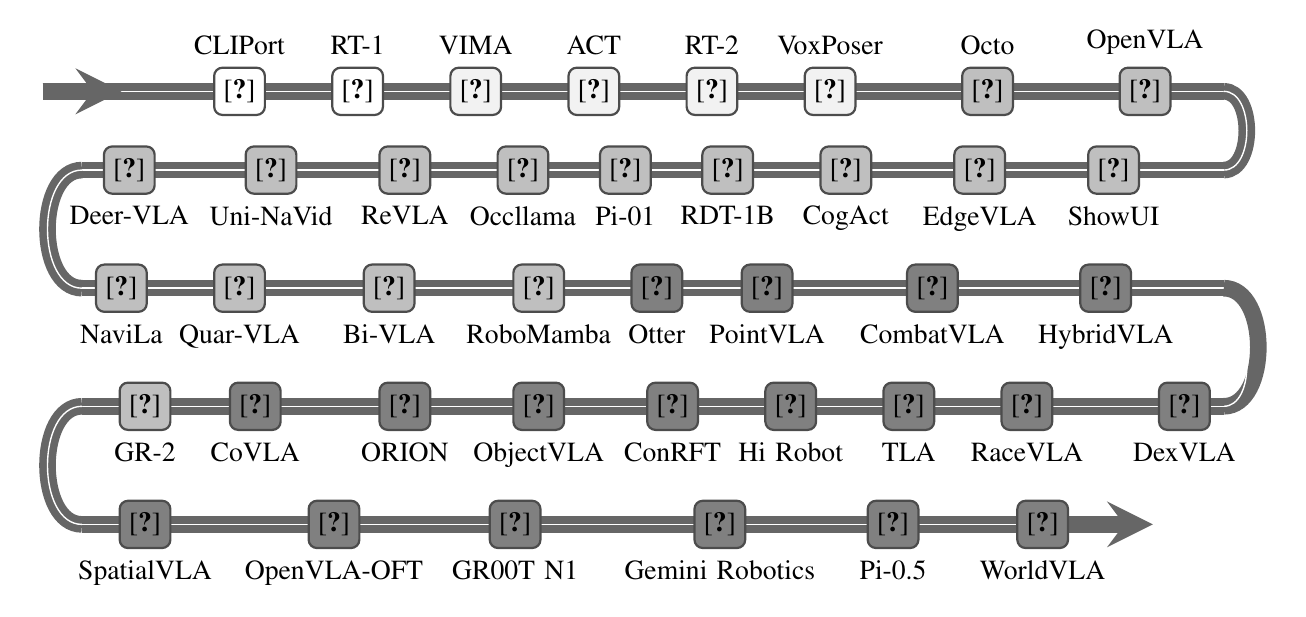
\begin{tikzpicture}[
  timeline/.style={ultra thick, draw=black!60, rounded corners=3pt},
    label/.style={align=center,  text width=2.3cm, inner sep=1pt},
    label2/.style={align=center,  text width=3cm, inner sep=1pt},
    event2022/.style={rounded corners=3pt, draw=black!70, fill=white, thick, minimum size=6mm, align=center, text=black},
    event2023/.style={rounded corners=3pt, draw=black!70, fill=gray!10, thick, minimum size=6mm,  align=center, text=black},
    event2024/.style={rounded corners=3pt, draw=black!70, fill=gray!50, thick, minimum size=6mm, align=center, text=black},
    event2025/.style={rounded corners=3pt, draw=black!70, fill=gray, thick, minimum size=6mm, align=center, text=black}
    ]

    % Main timeline path with reduced vertical spacing
    \draw[timeline,line width=6pt] (0,0) -- (15,0);
    \draw[-, line width=0.5pt, draw=white] (0,0) -- (15,0);
    % Arrow head at (0,0)
    \draw[-stealth, line width=6pt, draw=black!60] (0,0) -- (1,0);
    \draw[timeline,line width=6pt] (15,0) to[out=-0, in=0] (15,-1);
    \draw[-, line width=0.5pt, draw=white] (15,0) to[out=-0, in=0] (15,-1);
    \draw[timeline,line width=6pt] (15,-1) -- (0.5,-1);
    \draw[-, line width=0.5pt, draw=white] (15,-1) -- (0.5,-1);
    \draw[timeline,line width=6pt] (0.5,-1) to[out=-180, in=180] (0.5,-2.5);
    \draw[-, line width=0.5pt, draw=white] (0.5,-1) to[out=-180, in=180] (0.5,-2.5);
    \draw[timeline,line width=6pt] (0.5,-2.5) -- (15,-2.5);
    \draw[-, line width=0.5pt, draw=white] (0.5,-2.5) -- (15,-2.5);
    \draw[timeline,line width=6pt] (15,-2.5) to[out=-0, in=0] (15,-4);
    \draw[-, line width=0.5pt, draw=white] (15,-3) to[out=-0, in=0] (15,-4);
    \draw[timeline,line width=6pt] (15,-4) -- (0.5,-4); 
    \draw[-, line width=0.5pt, draw=white] (15,-4) -- (0.5,-4);
    \draw[timeline,line width=6pt] (0.5,-4) to[out=-180, in=180] (0.5,-5.5);
    \draw[-, line width=0.5pt, draw=white] (0.5,-4) to[out=-180, in=180] (0.5,-5.5);
    \draw[timeline,line width=6pt] (0.5,-5.5) -- (12.9,-5.5);
    \draw[-, line width=0.5pt, draw=white] (0.5,-5.5) -- (12.9,-5.5);
    \draw[-stealth, line width=6pt, draw=black!60] (12.9,-5.5) -- (14.1,-5.5);

    %%% Foundation Models %%%
    \node[event2022] (cliport) at (2.5,0) {\cite{shridhar2022cliport}};
    \node[label, above=3pt of cliport] {CLIPort};
    
    % \node[event2022] (gato) at (2.5,0) {\cite{reed2022generalist}};
    % \node[label, above=3pt of gato] {Gato};
    
    \node[event2022] (rt1) at (4,0) {\cite{rt-1}};
    \node[label, above=3pt of rt1] {RT-1};
    
    \node[event2023] (vima) at (5.5,0) {\cite{jiang2023vima}};
    \node[label, above=3pt of vima] {VIMA};
    
    \node[event2023] (act) at (7,0) {\cite{zhao2023learningFB}};
    \node[label, above=3pt of act] {ACT };
    
    \node[event2023] (rt2) at (8.5,0) {\cite{rt-2}};
    \node[label, above=3pt of rt2] {RT-2 };
    
    \node[event2023] (voxtposer) at (10,0) {\cite{huang2023voxposer}};
    \node[label, above=3pt of voxtposer] {VoxPoser };
    
    % \node[event2023] (diffpolicy) at (11.5,0) {\cite{chi2023diffusionpolicy}};
    % \node[label, above=3pt of diffpolicy] {Diffusion Policy };
    
    \node[event2024] (octo) at (12,0) {\cite{team2024octo}};
    \node[label, above=3pt of octo] {Octo };
    
    \node[event2024] (openvla) at (14,0) {\cite{kim2024openvla}};
    \node[label, above=3pt of openvla] {OpenVLA };

    %%% Specialized Applications %%%
    \node[event2024] (deer) at (1.1,-1) {\cite{yue2024deer}};
    \node[label, below=3pt of deer] {Deer-VLA };
    
    \node[event2024] (uni) at (2.9,-1) {\cite{zhang2024uni}};
    \node[label, below=3pt of uni] {Uni-NaVid };
    
    \node[event2024] (revla) at (4.6,-1) {\cite{dey2024revla}};
    \node[label, below=3pt of revla] {ReVLA };

    \node[event2024] (occllama) at (6.1,-1) {\cite{wei2024occllama}};
    \node[label, below=3pt of occllama] {Occllama };

    \node[event2024] (pi0) at (7.4,-1) {\cite{black2024pi_0}};
    \node[label, below=3pt of pi0] {Pi-01 };

    \node[event2024] (rdt) at (8.7,-1) {\cite{liu2024rdt}};
    \node[label, below=3pt of rdt] {RDT-1B };

    \node[event2024] (cogact) at (10.2,-1) {\cite{li2024cogact}};
    \node[label, below=3pt of cogact] {CogAct };

    \node[event2024] (edgevla) at (11.9,-1) {\cite{budzianowski20edgevla}};
    \node[label, below=3pt of edgevla] {EdgeVLA };

    \node[event2024] (showui) at (13.6,-1) {\cite{lin2024showui}};
    \node[label, below=3pt of showui] {ShowUI };

    %%% Robotics Focus %%%
    \node[event2024] (navila) at (1, -2.5) {\cite{cheng2024navila}};
    \node[label, below=3pt of navila] {NaviLa};

    \node[event2024] (quar) at (2.5, -2.5) {\cite{ding2024quar}};
    \node[label, below=3pt of quar] {Quar-VLA};

    \node[event2024] (bivla) at (4.4, -2.5) {\cite{gbagbe2024bi}};
    \node[label, below=3pt of bivla] {Bi-VLA};

    \node[event2024] (robomamba) at (6.3, -2.5) {\cite{liu2024robomamba}};
    \node[label, below=3pt of robomamba] {RoboMamba};

    \node[event2025] (otter) at (7.8, -2.5) {\cite{huang2025otter}};
    \node[label, below=3pt of otter] {Otter};

    \node[event2025] (pointvla) at (9.2, -2.5) {\cite{li2025pointvla}};
    \node[label, below=3pt of pointvla] {PointVLA};

    \node[event2025] (combatvla) at (11.3, -2.5) {\cite{chen2025combatvla}};
    \node[label, below=3pt of combatvla] {CombatVLA};

    \node[event2025] (hybridvla) at (13.5, -2.5) {\cite{liu2025hybridvla}};
    \node[label, below=3pt of hybridvla] {HybridVLA};

    %%% General Capabilities %%%
    \node[event2025] (covla) at (2.7, -4) {\cite{arai2025covla}}; % Changed from -6 to -5.2
    \node[label, below=3pt of covla] {CoVLA};
    % \node[event2025] (opendrivevla) at (2.7, -4) {\cite{zhou2025opendrivevla}}; % Changed from -6 to -5.2
    % \node[label, below=3pt of opendrivevla] {OpenDriveVLA};

    \node[event2025] (orion) at (4.6, -4) {\cite{fu2025orion}}; % Changed from -6 to -5.2
    \node[label, below=3pt of orion] {ORION};
    
    \node[event2025] (objectvla) at (6.3, -4) {\cite{zhu2025objectvla}}; % Changed from -6 to -5.2
    \node[label, below=3pt of objectvla] {ObjectVLA };

    \node[event2025] (conrft) at (8, -4) {\cite{chen2025conrft}}; % Changed from -6 to -5.2
    \node[label, below=3pt of conrft] {ConRFT};

    \node[event2025] (hirobot) at (9.5, -4) {\cite{shi2025hi}}; % Changed from -6 to -5.2
    \node[label, below=3pt of hirobot] {Hi Robot};

    \node[event2025] (tla) at (11, -4) {\cite{hao2025tla}}; % Changed from -6 to -5.2
    \node[label, below=3pt of tla] {TLA};
    
    \node[event2025] (racevla) at (12.5, -4) {\cite{serpiva2025racevla}}; % Changed from -6 to -5.2
    \node[label, below=3pt of racevla] {RaceVLA};

    \node[event2025] (dexvla) at (14.5, -4) {\cite{wen2025dexvla}}; % Changed from -6 to -5.2
    \node[label, below=3pt of dexvla] {DexVLA};
    %%% Newest Generalist Models (Q1--Q2 2025) %%%
    \node[event2024] (gr2) at (1.3, -4) {\cite{cheang2024gr2}};
    \node[label, below=3pt of gr2] {GR-2};

    \node[event2025] (spatialvla) at (1.3,-5.5) {\cite{qu2025spatialvla}};
    \node[label, below=3pt of spatialvla] {SpatialVLA};

    \node[event2025] (openvlaoft) at (3.7,-5.5) {\cite{openvla_oft}};
    \node[label2, below=3pt of openvlaoft] {OpenVLA-OFT};

    \node[event2025] (grootn1) at (6,-5.5) {\cite{gr00tn1}};
    \node[label, below=3pt of grootn1] {GR00T N1};

    \node[event2025] (geminirobotics) at (8.6,-5.5) {\cite{geminirobotics2025}};
    \node[label2, below=3pt of geminirobotics] {Gemini Robotics};

    \node[event2025] (pi05) at (10.8,-5.5) {\cite{pi05_2025}};
    \node[label, below=3pt of pi05] {Pi-0.5};

    \node[event2025] (worldvla) at (12.7,-5.5) {\cite{cen2025worldvla}};
    \node[label, below=3pt of worldvla] {WorldVLA};\end{tikzpicture}
}
\vspace{-1ex}
\caption{\scriptsize Recent robotic VLA models from {\fcolorbox{black}{white}{\scriptsize \text{2022}}} to {\fcolorbox{black}{gray}{\scriptsize \text{2025}}}.}\vspace{-1ex}
\label{fig:vla-timeline}
%   \end{minipage}
  \vspace{-2ex}
\end{wrapfigure}
% {\vspace{-1ex}} 
\BfPara{End-to-end Robotic Learning}
Building generalist
robots advances in multiple dimensions: 
\cib{1} the development and integration of vision, language, large action models, and multimodal fusion techniques into robotic learning, 
\cib{2} {\xo}-embodiment sensing and training using large, diverse datasets from across embodiments, enhanced transfer learning methods, and scalable data collection frameworks, and
\cib{3} the incorporation of real-time feedback, reinforcement learning on modular robotic models for various tasks.
High-capacity models have demonstrated an exceptional ability to process and learn diverse and extensive datasets, which is critical for end-to-end robotic learning. 
These models leverage their vast parameter space, \eg GPT-3, Jurassic-1, WuDao-2 with 175B+, Microsoft and Nvidia's Megatron-Turing NLG with 530B, and Google's Switch Transformer with 1.56 trillion parameters, to capture intricate patterns and relationships within the data, enabling them to generalize effectively across a wide array of tasks. 
Compared to these models, models used for robotic learning directly are relatively smaller, \eg RT-1~\cite{rt-1}, MOO~\cite{stone2023open}, and CLIPort~\cite{shridhar2022cliport} (with CLIP-ViT-Base), have 35M+, 111M, and 400M+, respectively. RT-2~\cite{rt-2} and variations of RT-2-X~\cite{9} incorporate pre-trained VLMs, which have large parameter space (\eg RT-2-PaLM-E and RT-2-PaLI-X have 12B and 55B, respectively).
Scaling up these models faces many challenges: 
\cib{1} maintaining real-time inference under strict time constraints (\eg 3-5Hz), 
\cib{2} maintaining robustness and coherence when generalizing to novel tasks and environments, 
\cib{3} addressing the computational demands and resource requirements of training and deployment, 
\cib{4} managing the complexity of integrating multimodal inputs, and 
\cib{5} ensuring reliability and safety in dynamic and unpredictable real-world settings.
As end-to-end techniques and integration of large vision, LLM, and VLM backbones become more prevalent~\cite{9} (see the evolution of robotic models in \autoref{fig:vla-timeline}), security research for these models is limited. Generalist robotic models continue to emerge, \eg OpenVLA-OFT, {GR00T}~N1, Gemini Robotics, pi-0.5, and WorldVLA~\cite{qu2025spatialvla,openvla_oft,gr00tn1,geminirobotics2025,pi05_2025,cen2025worldvla,cheang2024gr2}. Ensuring these models resilience to attacks is crucial.
To this end, we identify the following challenges.
% We identify the key challenges in ensuring model resilience to adversarial attacks.


\BfPara{C1: Wide-array of Data and Model Adoption}
The emergence of large-scale datasets for {\xo}-embodied generalist robots across diverse robotic platforms, embodiments, and environments has enabled many advances in the field.
Standardizing and processing these heterogeneous datasets in a consistent format requires substantial effort and innovation, as seen in efforts such as RoboNet~\cite{dasari2020robonet} and Open {\xo}-Embodiment Repository~\cite{9}. 
These datasets cover different kinds of tasks, objects, scenarios, and settings.
Moreover, recent work showed the benefits of learning visual representations from human video data~\cite{nair2022r3m,xiao2022masked,radosavovic2022,majumdar2024we,karamcheti2023language,mu2023ec2,bahl2023affordances} for robotics learning. 
Beyond robot-specific or {\xo}-embodied data, more data will inevitably be included to train generalist models.
This introduces security/safety challenges that must be addressed to prevent/mitigate vulnerabilities.


\BfPara{C2: Multimodal Data and Model Integration} 
The integration of multimodal data, \ie vision, language, and action, into large foundation models for robotics presents substantial security complexities. 
Despite the importance of this integration to improve robot functionality and autonomy through understanding and interacting with unseen environments, the heterogeneous nature of multimodal data greatly increases the attack surface, offering multiple avenues for malicious interference. 
Each data modality introduces particular vulnerabilities; for instance, adversarial images can fool vision models, while subtly changed text inputs can fool language models. Moreover, it is more challenging to determine the impact of adversarial manipulations on input data due to the varied ways in which such data and models are used in end-to-end robot learning.
We must identify and counteract attacks that can exploit the specific weaknesses of each modality. 


\BfPara{C3: Robustness and Trustworthiness}
Ensuring the robustness and trustworthiness of robotic agents is a major challenge. 
Few studies have adequately assessed factors such as interpretability, robustness, safety, and fairness in robots, raising concerns about the potential for inherited vulnerabilities and bias from large backbone models. We must assess robot models
under a variety of conditions, including adversarial attacks and unexpected inputs, and develop methods that can improve their robustness.
We must develop methods for interpretability and fairness to ensure transparent and unbiased decisions.


These challenges represent a tremendous opportunity for research into end-to-end learning models for {\xo}-embodied generalist robots. The PIs are well-positioned to advance this field through their expertise in AI security, robust model development, robotic systems, and distributed modeling and analysis.

\begin{comment}
    
\BfParaUL{Team}
\textbf{PI Abuhamad}
PI Abuhamad is an expert in AI security, especially in the security of large models. 
The PI has led significant work on secure and reliable AI systems~\cite{abuhamad2018large,abuhamad2020autosen,alasmary2020soteria,abuhamad2020multi,abusnaina2021dl,abuhamad2021large,abdukhamidov2023hardening,juraev2024unmasking,juraev2024impact,alawami2024motionid,abdukhamidov2024singleadv}, developing novel approaches to secure and interpretable AI \cite{abdukhamidov2023hardening,abusnaina2021dl,abdukhamidov2024singleadv,abdukhamidov2025stealthy,abuhamad2025nlp,abuhamad2025vit}, software security~\cite{abuhamad2018large,abuhamad2018large,abuhamad2020multi}, online security, privacy and safety~\cite{khan2023identification,reyes2023webtracker,shao2023lightweight,abuhamad2025shield}, and secure authentication methods~\cite{abuhamad2020autosen,alawami2024motionid}. 
These works appeared in ACM CCS, IEEE ICDCS, IEEE TDSC, ACM TOPS, IEEE TIFS, IEEE IoT-J, and PoPETS.  Because of this background and prior work, PI Abuhamad is uniquely positioned to carry out the proposed work.
\textbf{PI Thiruvathukal}
%TODO Add PI Thiruvathukal's relevant publications and contributions.

The PIs recognize the vast and evolving landscape of adversarial attacks against large foundation models. 
In this project, the PIs will work to establish foundational research and collaborative efforts to develop comprehensive frameworks and benchmarks that build toward secure and reliable robotic models. 
%While addressing all possible attack vectors is impossible within a single project, creating foundational tools, metrics, and methodologies will enable the broader research community to systematically evaluate and improve robotic system security. 
%The PI will leverage expertise in AI security to create lasting infrastructure that supports continuous improvement in robotic model security, with a particular focus on developing standardized evaluation protocols that can evolve alongside emerging threats.

\end{comment}





\subsection{Vulnerability Analysis in Foundation Generalist Robots}

This proposal aims to secure emerging robotic foundation models, where security and robustness are crucial.
Based on the NIST Trustworthy and Responsible AI report~\cite{NIST_AI_100_2e2023}, the taxonomy of the most studied and effective attacks includes \emph{evasion}, \emph{poisoning}, \emph{privacy}, and \emph{abuse} attacks. % for generative AI systems.
For end-to-end robotic models, this proposal addresses all categories of attacks (\autoref{table:attacks_models}).%, including evasion, poisoning, privacy, and abuse attacks.
% Given the high-dimensional and multimodal nature of the search space for attacks aginst robotic models, simply introducing random noise to inputs might fail to identify subtle vulnerabilities of the robotic model.
% Moreover, robotic models/policies are generally designed to be resilient against such noise~\cite{miki2022scirob}, making such adversarial attacks ineffective using straightforward methods.

\BfPara{Challenges} 
Attacking robotic models
presents unique challenges due to their complex architectures, the multimodal nature of their input, restrictions on the output/action space, and the evolving landscape of security measures. 
Main challenges include the following:
{\cib{1}} \emph{{Multimodal Complexity}:} Generalist robotic models process/integrate data from multiple modalities, such as sensory/positions data, images, and text, to predict action sequences. %We believe that the efforts to build robotic foundation models will continue to grow and other modalities will be incorporated.
    % Creating effective attacks requires understanding and manipulating the intricate relationships and interactions among these modalities \cite{radford2021learning}. 
    % Consequently, 
    Creating adversarial examples that can deceive both the visual and language components is more challenging than focusing on one. 
{\cib{2}} \emph{{Model Scale and Complexity:}} Current robotic models involve large architectures containing millions to billions of parameters, making them highly complex and computationally expensive to attack.
    Examining adversarial attacks on such large models necessitates significant computational resources.
{\cib{3}} \emph{{Attack Practicality and Transferability:}} 
    Adversarial scenarios against robotics should be practical, \ie scenarios in which robots are likely to face operational tasks. 
Therefore, attacks must be systematic and guided by practical experience in field robotics to ensure the plausibility and reflection of real-world scenarios. 
    Moreover, attack methods against similar LLMs/VLMs use white-,
\begin{wraptable}{r}{0.4\textwidth}
\centering 
\vspace{-2.5ex}
\caption{{\footnotesize Stages (Training and Inference), targets (Privacy, Integrity, Availability, and Abuse) and types ( White- (\dd), Gray- (\bb), and Black-box (\vv) ) of common Evasion, Poisoning, and Privacy attacks.}}\vspace{-2.5ex}
\label{table:attacks_models}
\small
\resizebox{0.92\linewidth}{!}{%
\begin{tblr}{
rowsep=0pt,
column{1} = {c,0.1cm},
  column{3} = {c,0.15cm},
  column{4} = {c,0.15cm},
  column{5} = {c,0.15cm},
  column{6} = {c,0.15cm},
  column{7} = {c,0.15cm},
  column{8} = {c,0.15cm},
  column{9} = {c,0.15cm},
  cell{2}{1} = {r=8}{},
  cell{10}{1} = {r=10}{},
  cell{20}{1} = {r=6}{},
  hline{2,10,20,26} = {-}{},
}
                                                  &                                & \begin{sideways}{\rotatebox{-45} {Training}}\end{sideways} & \begin{sideways}{\rotatebox{-45} {Inference}}\end{sideways} & \begin{sideways}{\rotatebox{-45} {Privacy}}\end{sideways} & \begin{sideways}{\rotatebox{-45} {Integrity}}\end{sideways} & \begin{sideways}{\rotatebox{-45} {Availability}}\end{sideways} & \begin{sideways}{\rotatebox{-45} {Abuse}}\end{sideways} & \begin{sideways}{\rotatebox{-45} {Type}}\end{sideways} \\
\begin{sideways}Evasion      ~\end{sideways}      & Indirect Prompt Injection      & \ee                                       & \checkmark                                         & \checkmark                                       & \checkmark                                         & \checkmark                                            & \checkmark                                     & \vv                          \\
                                                  & Universal Adversarial Triggers & \ee                                       & \checkmark                                         & \ee                                      & \ee                                        & \ee                                           & \checkmark                                     & \vv                          \\
                                                  & Gradient-based Attacks         & \checkmark                                        & \checkmark                                         & \ee                                      & \ee                                        & \ee                                           & \ee                                    & \dd                          \\
                                                  & Prompt Injection               & \ee                                       & \checkmark                                         & \checkmark                                       & \checkmark                                         & \checkmark                                            & \checkmark                                     & \bb                           \\
                                                  & Refusal Suppression            & \ee                                       & \checkmark                                         & \ee                                      & \ee                                        & \ee                                           & \checkmark                                     & \bb                           \\
                                                  & Style Injection                & \ee                                       & \checkmark                                         & \ee                                      & \ee                                        & \ee                                           & \checkmark                                     & \bb                           \\
                                                  & Role-play Strategies           & \ee                                       & \checkmark                                         & \ee                                      & \ee                                        & \ee                                           & \checkmark                                     & \bb                           \\
                                                  & Jailbreak           & \ee                                       & \checkmark                                         & \ee                                      & \ee                                        & \ee                                           & \checkmark                                     & \bb                           \\
\begin{sideways}Poisoning         ~\end{sideways} & Data Poisoning                 & \checkmark                                        & \ee                                        & \ee                                      & \checkmark                                         & \checkmark                                            & \ee                                    & \dd                          \\
                                                  & Model Poisoning                & \checkmark                                        & \ee                                        & \ee                                      & \checkmark                                         & \checkmark                                            & \ee                                    & \dd                          \\
                                                  & Backdoor Poisoning             & \checkmark                                        & \checkmark                                 & \checkmark                                 & \checkmark                                        & \ee                                           & \checkmark                                     & \dd                          \\
                                                  & Label Flipping                 & \checkmark                                        & \ee                                        & \ee                                      & \checkmark                                         & \checkmark                                            & \ee                                    & \dd                          \\
                                                  & Clean-label Poisoning          & \checkmark                                        & \ee                                        & \ee                                      & \checkmark                                       & \ee                                           & \ee                                    & \dd                          \\
                                                  & Targeted Poisoning             & \checkmark                                        & \ee                                        & \ee                                      & \checkmark                                        & \ee                                           & \ee                                    & \dd                          \\
                                                  & Subpopulation Poisoning        & \checkmark                                        & \ee                                        & \ee                                      & \checkmark                                       & \ee                                           & \ee                                    & \dd                          \\
                                                  & Model Replacement              & \checkmark                                        & \ee                                        & \ee                                      & \checkmark                                        & \ee                                           & \ee                                    & \dd                          \\
                                                  & Model Boosting                 & \checkmark                                        & \ee                                        & \ee                                      & \checkmark                                        & \ee                                           & \ee                                    & \dd                          \\
                                                  & Functional Attacks             & \checkmark                                        & \ee                                        & \ee                                      & \checkmark                                        & \ee                                           & \ee                                    & \dd                          \\
\begin{sideways}Privacy\end{sideways}             & Data Reconstruction            & \ee                                       & \checkmark                                         & \checkmark                                       & \ee                                        & \ee                                           & \ee                                    & \vv                          \\
                                                  & Membership Inference           & \ee                                       & \checkmark                                         & \checkmark                                       & \ee                                        & \ee                                           & \ee                                    & \bb                           \\
                                                  & Model Extraction               & \ee                                       & \checkmark                                         & \checkmark                                       & \ee                                        & \ee                                           & \ee                                    & \vv                          \\
                                                  & Property Inference             & \ee                                       & \checkmark                                         & \checkmark                                       & \ee                                        & \ee                                           & \ee                                    & \bb                           \\
                                                  & Attribute Inference            & \ee                                       & \checkmark                                         & \checkmark                                       & \ee                                        & \ee                                           & \ee                                    & \bb                           \\
                                                  & Prompt and Context Stealing    & \ee                                       & \checkmark                                         & \checkmark                                       & \ee                                        & \ee                                           & \ee                                    & \vv                          
\end{tblr}
}{\vspace{-3ex}}
\end{wraptable}%\vspace{-5ex}
    gray-, and black-box settings relying on prior knowledge of (exact or similar) models, training data, restrictions/constraints of the system or training a surrogate models. However, robotic applications and commercial vendors often do not share model details \cite{cheng2018query}. In practice, attackers can only query the model and observe the behavior of the robot/output of the model. Developing attacks that exploit multiple vulnerabilities \cite{biggio2018wild} or adapt to various threat vectors is necessary and requires various strategies.
    Numerous studies have shown that some attacks exhibit high transferability, \ie attacks on a given model can succeed on other similar models. This phenomenon derived the transfer-based black-box attacks.
    Nevertheless, attacks designed for similar LLMs/VLMs models might not always work effectively on other models, even if they share similar architectures. 
    Ensuring adversarial examples are transferable \cite{liu2016delving} across models and tasks requires understanding model-specific vulnerabilities and generalizable attack methods.
\\
\BfPara{Definitions: Attacking Robotic Foundation Models}
{Let $\mathcal{F}$ represent a robotic foundation model, which takes a tuple of inputs, \eg $(\{\bm{x}\}, \{\bm{t}\}, \{\bm{s}\}, \dots)$ representing input modalities (\ie a set (at least one) of images \{$\bm{x}\} \in \mathcal{X}$, set of text instructions $\{\bm{t}\} \in \mathcal{T}$, set of sensory/position data $\{\bm{s}\}\in \mathcal{S}$, and other available information) and outputs a set of tokenized actions $\mathcal{F}(\{\bm{x}\}, \{\bm{t}\}, \{\bm{s}\}, \dots)=\{\bm{a}_{out}\}$.
Since robots could have multiple embodiments/tasks (and various action spaces), some inputs could become a placeholder/masked $\oslash$ or nonexistent input to fit the model.}
For example, RT-2 and OpenVLA models receive only images and textual instruction $\mathcal{F}(\{\bm{x}\}, \{\bm{t}\})=\{\bm{a}_{out}\}$, 
Octo receives images, text, and sensory data $\mathcal{F}(\{\bm{x}\}, \{\bm{t}\}, \{\bm{s}\})=\bm{a}_{out}$, and ACT receives only images and sensory data $\mathcal{F}(\{\bm{x}\}, \{\bm{s}\})=\{\bm{a}_{out}\}$.
If Octo is used for robots/datasets that do not provide text instructions, the model processes available inputs and masks unavailable ones $\mathcal{F}(\{\bm{x}\}, \oslash,\{\bm{s}\})=\{\bm{a}_{out}\}$.
The output $\{\bm{a}_{out}\}$ is one or chunks of actions, each is a sequence of tokens representing predicted actions.



The attack operation $\mathcal{M}(.)$ is defined as a perturbation function that alters the inputs (one or more 
modalities) to mislead the model into producing an incorrect/unintended output action.
For example, $\mathcal{M}(\bm{x})$ attacks image inputs $\bm{x}$, $\mathcal{M}(\bm{t})$ attacks text inputs $\bm{t}$, and $\mathcal{M}(\bm{x}, \bm{t})$ attacks both images and instructions.
\ul{\emph{Adversarial specificity}} can be either \textbf{targeted} or \textbf{untargeted} against security concepts. % \emph{Integrity}, \emph{Confidentiality}, and \emph{Availability}.
The \ul{\emph{attacks goals}} can be categorized into \textbf{evasion}, \textbf{poisoning}, and \textbf{privacy}, and can be \ul{launched either in \textbf{training} or \textbf{inference} phases}.
For example, $\mathcal{M}(\bm{x},\bm{t}) \xrightarrow{{}_{\textbf{U}}} \bm{a}_{out}'$ such that $\bm{a}_{out}' \neq \bm{a}_{out}$ is an untargeted evasion attack that alters the input pair $(\bm{x},\bm{t})$ to cause the model to produce an incorrect output $\bm{a}_{out}'$.
Similarly, $\mathcal{M}(\bm{t}) \xrightarrow{{}_{\textbf{T}}} \bm{a}_{jailbreak}$ is a targeted jailbreak attack that alters the input instructions to cause the model to produce a specific (undesired) output.
If the attack is designed such that $\mathcal{M}(\bm{x},\bm{t}) \xrightarrow{{}_{\textbf{U}}} \bm{a}_{out}'$ where $\bm{a}_{out}'$ reveals confidential information, this constitutes a privacy attack.
Depending on the level of the \ul{\emph{adversary's capabilities and knowledge}} on the victim model/data/system, adversarial attacks can be categorized into \textbf{white-box}, \textbf{gray-box}, and \textbf{black-box} attacks. 
% \autoref{table:attacks_models} shows the general adversarial attack on robotic models.
Several threat models can be defined based on the adversarial specificity/goals, timing of the attack (\eg training or inference), the extent of adversarial capabilities, and the knowledge about the target model/system (\eg model parameters, source code, and/or training data).






\newpage
\section{Research Plan}

This work proposes a novel security framework for end-to-end generalist robots to address the inherent challenges of ensuring robustness, security, and trustworthiness in general-purpose robots across various physical embodiments. 
End-to-end generalist robot models leverage high-capacity models (\eg ViTs, LLMs, VLMs, and VLAs) pre-trained using Internet-scale data and training pipelines that use specific and/or \xot robotics datasets. 
The core concept relies on the systematic evaluation and discovery of potential vulnerabilities in all layers of the robotic learning stack. This plan describes the research tasks in this project.


\subsection{T0: Ongoing Progress: Comprehensive Repository for Robotic Models and Data} \label{sec:t0}
% ~\vspace{-3ex}
\begin{wraptable}{r}{0.5\textwidth}\vspace{-2.5ex}
% \begin{table}
\centering
\caption{{Datasets augmenting OXE~\cite{9} for robots (\textbf{R}), \textbf{F}ranka, \textbf{G}oogle Robot, \textbf{S}pot, \textbf{H}ello Stretch, \textbf{U}R5, Hu\textbf{M}an}, and \textbf{X}arm7, with control frequency (\textbf{Hz}) and \textbf{\#} of episodes.}
\label{tab:multi_dataset}\vspace{-2ex}
\resizebox{0.97\linewidth}{!}{%
\begin{tabular}{p{4cm}ccp{4cm}c}
\toprule
Dataset                     & \textbf{R}         &\textbf{ \#} & {Action Space}                           & \textbf{Hz}           \\
\midrule
 Franka  \cite{rosete2022tacorl,mees23hulc2}        & F       & 3242        & EEF Position                           & 15                            \\
Maniskill     \cite{gu2023maniskill2}               & F        & 30000       & EEF Position                           & 20                                               \\
Robocook   \cite{shi2023robocook}        & F       & 2460        & EEF Position                           & 5                                                \\
CMU Pick-Insert \cite{saxena2023multiresolution} & F        & 520         & EEF Position                           & 20                                      \\
RoboVQA  \cite{9}                       & G  & 61153       & EEF Position                           & 10                                                     \\
DROID \cite{khazatsky2024droid}                         & F        & 92233       & EEF Position                           & 15                                          \\
ConqHose  \cite{ConqHoseManipData}                     & S          & 139         & EEF velocity                           & 30                                          \\
DobbE   \cite{shafiullah2023dobbe}                     & H & 5208        & EEF Position                           & 3.75                                        \\
FMB \cite{luo2024fmb}                           & F        & 1804        & EEF velocity                           & 10                                                  \\
IO-AI Office \cite{9}    & M        & 3847        & EEF Position                           & 30                                                       \\
RoboSet\cite{bharadhwaj2023roboagent}                     & F        & 18250       & Joint position                         & 5                                        \\
VIMA \cite{jiang2023vima}                        & U          & 660103      & Primitive skills                       & NA                                               \\
SPOC \cite{spoc2023}                       & H & 233000      & Joint position                         & 10                                                     \\
Ours & X & 10000 & EEF/joint Position & 5-50 \\
\bottomrule
\end{tabular}}\vspace{-2ex}
\end{wraptable}
To conduct research tasks toward assessing and enhancing robustness, trustworthiness, and performance of robotic foundation models, we are  building/training/evaluating various models using state-of-the-art techniques and \xot data.\\
\BfPara{Robotics Data Mixture} We consider a multimodal robotics data mixture of
six robot embodiments (Franka, Google Robot, Spot, Hello Stretch, UR5, and Xarm7; \textit{fewer than the 22 embodiments in the OXE~\cite{9} dataset, for multimodality and practical reasons}) in addition to human demonstration data (see \autoref{tab:multi_dataset}). The mixture draws from 15 dataset sources: 14 robotics datasets (\autoref{tab:multi_dataset}, including our own for Xarm7) and the Open X-Embodiment (OXE)~\cite{9} repository, which  aggregates 60 robotic datasets.
We plan to continue extending our dataset (\ie added tasks/episodes) as we continue in our research.% and this project. 




\BfPara{End-to-end Models}
We identify two main families of end-to-end robotic foundation models: policy prediction models (\eg VLAs) and goal-conditioned models (\eg RoboCat~\cite{bousmalis2023robocat}). VLAs predict the next action based on the current state and instruction, while the second family, goal-conditioned models, predicts the next state based on the current state and goal. VLAs are gaining more traction due to their ability to leverage large pre-trained models and fine-tune them for specific tasks/embodiments (see~\autoref{fig:vla-timeline}).
{In the following, we describe the main models that we will use in this project. We will continue to expand the list of models as new models are released and/or become available for research use.}

\noindent\textbf{\cib{1} RT-1~\cite{rt-1} and RT-1-X~\cite{9}:} RT-1 is a 35M parameter network built on a transformer architecture~\cite{vaswani2017attention} and designed for robotic control. 
It takes in a history of images (\eg 5 to 15 images) of resolution $300\times300$ along with the natural language instructions. 
Each image is processed through an ImageNet-pre-trained EfficientNet-B3~\cite{tan2019efficientnet} to output spatial feature maps of shape $9\times9\times512$ from the final convolutional layer.
The model was chosen primarily to balance accuracy, model size, and speed, keeping the local processing rate within 3Hz for the entire pipeline.
The natural language instruction is transformed into a USE~\cite{cer2018universal} embedding. 
The visual and language representations are then interwoven via FiLM~\cite{perez2017film} layers, producing 81 vision-language tokens. 
These tokens are fed into a decoder-only transformer that outputs the tokenized actions.
To tokenize actions, each action dimension in RT-1 is discretized into $256$~bins.
\begin{comment}
The action dimensions we consider include seven variables for the arm movement ($x$, $y$, $z$, roll, pitch, yaw, opening of the gripper), three variables for base movement ($x$, $y$, yaw), and a discrete variable to switch between three modes: controlling arm, base or terminating the episode.
For example, an action
``$\Delta \textit{pos}_x\text{=}0.1 \enspace \Delta \textit{pos}_y\text{=}-0.2 \enspace \Delta \textit{pos}_z\text{=}0 \enspace \Delta \textit{rot}_x\text{=}10^{\circ} \enspace \Delta \textit{rot}_y\text{=}25^{\circ} \enspace \Delta \textit{rot}_z\text{=}-7^{\circ}
$'' for the arm could be represented as ``\textit{132 114 128 5 25 156}''.
For each variable, the target action/value is mapped to a value from the 256 bins, where the bins are uniformly distributed within the bounds of each variable. The {loss}
used for RT-1 training is a standard categorical cross-entropy entropy and causal masking that was utilized in prior transformer-based controllers~\cite{reed2022generalist,lee2022multi}. 
\end{comment} 
We use the same implementation/design choices for RT-1 model as reported by the original work. Other variations of RT-1, \eg different base/backbone models, %and operation modes (\ie local or cloud-based inference), 
will be implemented as RT-1-X designs.


\noindent\textbf{\cib{2} RT-2~\cite{rt-2} and RT-2-X~\cite{9}:} RT-2 is a large (12--55B parameters) VLA model.
RT-2 casts the tokenized actions as text tokens.
As such, any pre-trained VLM (\eg Pali-X~\cite{chen2023palix}, Flamingo~\cite{alayrac2022flamingo}, {P}a{LM}-E~\cite{driess2023palme}) can be fine-tuned for robotic control.%, thus leveraging the backbone of VLMs and transferring some of their generalization properties.
Action encoding and discretization are performed as in \cite{rt-1} for the RT-1 model. 
% To fine-tune a VLM into a VLA model, tokens should be associated with the discrete action bins (\ie reserving 256 tokens to serve as action tokens). 
% In order to define a target for VLM fine-tuning, the action vector is represented by a single string that simply concatenates action tokens for each dimension with a space character:
% For example, a possible instantiation of the target,
% ``$\textit{terminate} \enspace \Delta \text{pos}_x \enspace \Delta \textit{pos}_y \enspace \Delta \textit{pos}_z \enspace \Delta \textit{rot}_x \enspace \Delta \textit{rot}_y \enspace \Delta \textit{rot}_z \enspace \textit{gripper\_extension}
% $'',
% could be: ``\textit{1 128 91 241 5 101 127}''.
To ensure that RT-2 outputs valid action tokens during decoding, the output vocabulary is
constrained to only sampling valid action tokens when the model is prompted with a robot-action task.
We note that the model, \ie the original VLM, can still output the full range of language tokens on standard vision-language tasks.
Our implementation focuses on RT-2-X variants with common open-source VLMs (see \autoref{tab:VLMs} for their components). 
\begin{wraptable}{r}{0.4\textwidth}
\centering
\vspace{-0.5ex}
\caption{{\footnotesize VLMs for RT-2-[X] and [X]-VLA Variants.}}
\label{tab:VLMs}
\vspace{-2ex}
\resizebox{\linewidth}{!}{
\begin{tabular}{llll}
\toprule
Model & LLM & Adapter & Vision \\ \midrule
Flamingo~\cite{alayrac2022flamingo} & Chinchilla & Attention & NFNet-F6 \\
OpenFlamingo~\cite{awadalla2023openflamingo} & MPT & Attention & CLIP ViT-L \\
SPHINX-X~\cite{gao2024sphinx} & Mixtral & Linear & Mixture \\
Qwen-VL~\cite{bai2023qwen} & Qwen & Q-Former & ViT-bigG \\
BLIP-2~\cite{li2023blip} & Flan-T5/OPT & Q-Former & EVA ViT-g \\
InstructBLIP~\cite{dai2024instructblip} & Vicuna & Q-Former & EVA ViT-g \\
BLIVA~\cite{hu2024bliva} & Vicuna & Q-Former & EVA ViT-g \\
MiniGPT-4~\cite{zhu2023minigpt} & Vicuna & Linear & EVA ViT-g \\
MiniGPT-v2~\cite{chen2023minigpt} & LLaMA-2 & Linear & EVA ViT-g \\
LLaVA~\cite{liu2024visual} & Vicuna & Linear & CLIP ViT-L \\
LLaVA-1.5~\cite{liu2024improved} & Vicuna-v1.5 & MLP & CLIP ViT-L \\
LLaMA Adapter-V2~\cite{gao2023llama} & LLaMA & Linear & CLIP ViT-L \\
PandaGPT~\cite{su2023pandagpt} & Vicuna & Linear & ImageBind \\
\bottomrule
\end{tabular}}\vspace{-2ex}
\end{wraptable}
\noindent\textbf{{\cib{3}} OpenVLA and [X]-VLA Variants:} 
OpenVLA~\cite{kim2024openvla} (7B parameters)
is an open-source alternative to RT-2~\cite{rt-2}. % that is built on the open-source VLMs.
OpenVLA, as other VLAs, follows the same design principles that include training/fine-tuning open-source VLMs which consist of three components: vision tokenizer/encoder/adapter, LLM backbone, and action decoder/tokenizer. 
OpenVLA uses Prismatic VLM (7B-parameter) and is trained on 970k real-world robot demonstrations outperforming larger models like RT-2 ($\sim$55B). The Prismatic VLM uses dual vision encoders (DINOv2 \cite{oquab2023dinov2} and SigLIP \cite{zhai2023sigmoid}) and a LLaMA-2 language model \cite{touvron2023llama}.
Variants of OpenVLA, \eg  ReVLA~\cite{dey2024revla}, Edge-VLA~\cite{budzianowski20edgevla}, PointVLA~\cite{li2025pointvla}, and CoVLA~\cite{arai2025covla} (see \autoref{fig:vla-timeline}), have been proposed to improve the original design in terms of performance, efficiency, reasoning, and/or specialty.
Similar to RT-2-X, we will adopt various open-source VLMs/components to build/train [X]-VLA variants.


% \noindent\textbf{\cib{4} RoboCat~\cite{bousmalis2023robocat}} RoboCat follows a different approach by conditioning the model on visual goal. The architecture is VQ-GAN encoder which is based on the Gato architecture~\cite{esser2021taming} that processes the image (with $128\times128$ resolution) as $8\times8$ tokens and outputs encoded vectors. These vectors are then discretized via a nearest-neighbor lookup in a codebook of embeddings.
% The VQ-GAN encoder is a ResNet~\cite{resnet} with 2 groups of 2 blocks, followed by 3 attention layers. 
% The decoder has 3 attention layers followed by a ResNet with 2 groups of 3 blocks. %The vector quantiser~\citep{van2017neural} uses 64 embeddings of dimension 128. 
% For tokenization of observations and actions, RoboCat follows a similar approach as~\cite{reed2022generalist}.
% The loss is weighted as ($0.25\times\text{discretization\_loss} + \text{l2\_reconstruction\_loss} + 0.1\times\text{log\_laplace\_loss}$) to predict future tokens. The output is the image tokens at time step $k = 5$, as one step can look very similar.

\noindent\textbf{\cib{4} Octo~\cite{team2024octo}:} Octo is a (27-93M parameters) transformer-based VLA pre-trained on the OXE~\cite{9} dataset. Unlike RT-X, it can be fine-tuned to new observations and action spaces. This flexibility allows Octo to adapt to various robotic embodiments, a trend that is becoming increasingly important/adopted in robotics.
Octo architecture consists of three key parts: \textit{input tokenizers} that transform language instructions and observations into tokens, a \textit{transformer backbone} that receives the tokens and generates embeddings, and \textit{readout heads} that produce the desired outputs, \ie actions. Input tokenizers include modality-specific tokenizers, \ie a language (task) tokenizer (\eg T5) and a vision tokenizer (\eg ViT-based or CNN-based). Unavailable modalities are masked (\eg no language instructions are provided), and learnable position embeddings are added to the input tokens before feeding them into the transformer backbone.  Octo also uses a \textit{readout token} analogous to the $\text{[CLS]}$ token in BERT/LLMs.
The transformer backbone processes the input tokens through block-wise masked attention patterns (\ie see to tokens from the same or earlier time steps), which are then passed to the readout heads. The readout ``\textit{action}'' head predicts a ``\textit{chunk}'' of several consecutive actions.
Action heads can be added/replaced/fine-tuned during fine-tuning (\eg adoption of new embodiments).
\begin{wrapfigure}{r}{0.4\textwidth}{\vspace{-2.5ex}}
  \centering
\begin{minipage}{0.4\textwidth}
      \centering
        \begin{minipage}{\linewidth}
          \centering
          \begin{minipage}{0.33\linewidth}
            \centering
            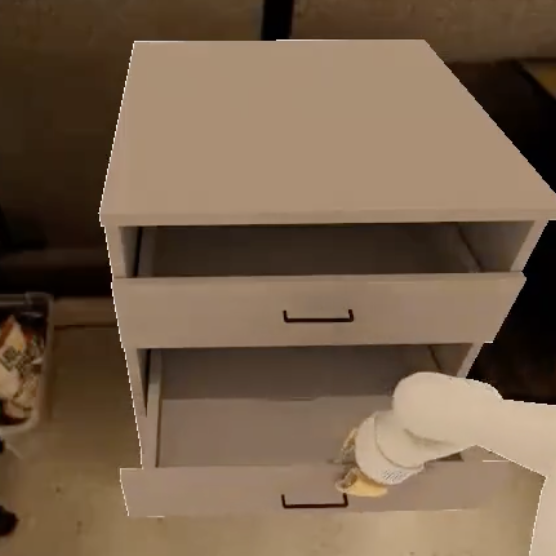
\includegraphics[width=\textwidth]{figures/examples/1.png}
          \end{minipage}%
          \begin{minipage}{0.33\linewidth}
            \centering
            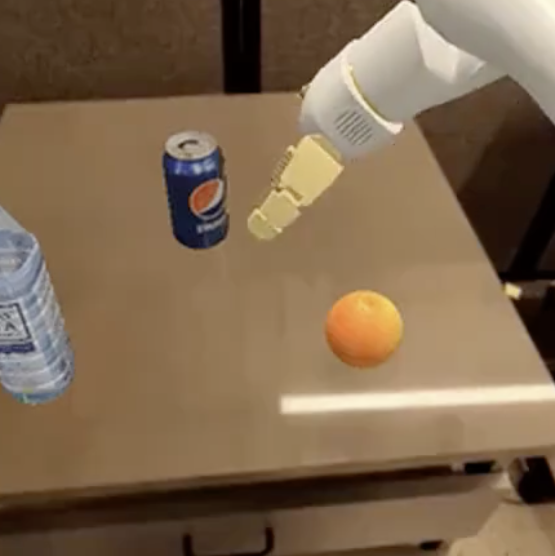
\includegraphics[width=\textwidth]{figures/examples/2.png}
          \end{minipage}%
          \begin{minipage}{0.33\linewidth}
            \centering
            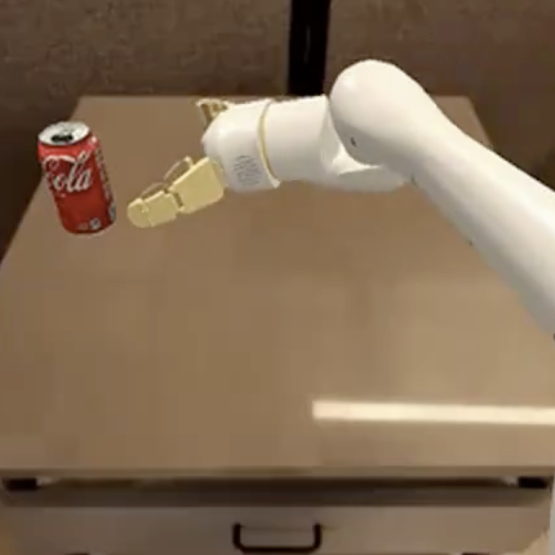
\includegraphics[width=\textwidth]{figures/examples/3.png}
          \end{minipage}
        \end{minipage}\vspace{-1.5ex}
        \begin{minipage}{\linewidth}
          \centering
          \begin{minipage}{0.33\linewidth}
            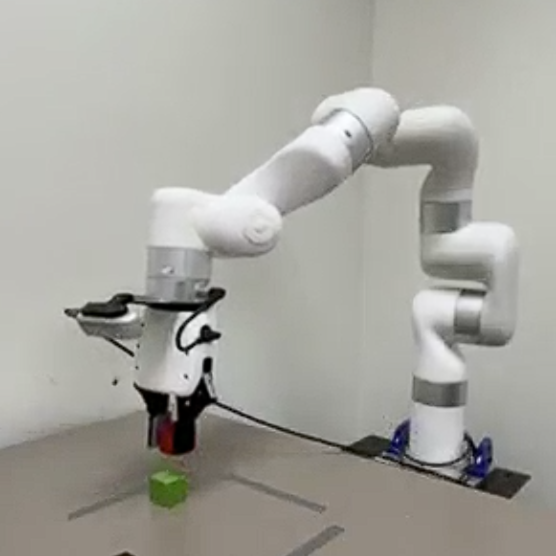
\includegraphics[width=\textwidth]{figures/examples/4.png}
          \end{minipage}%
          \begin{minipage}{0.33\linewidth}
              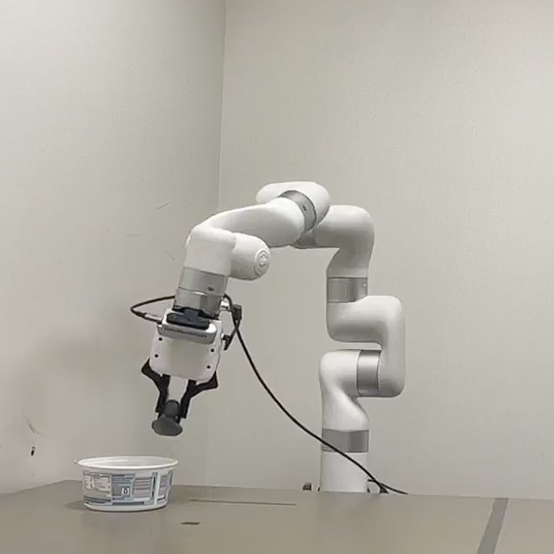
\includegraphics[width=\textwidth]{figures/examples/5.png}  
            \end{minipage}%
          \begin{minipage}{0.33\linewidth}
            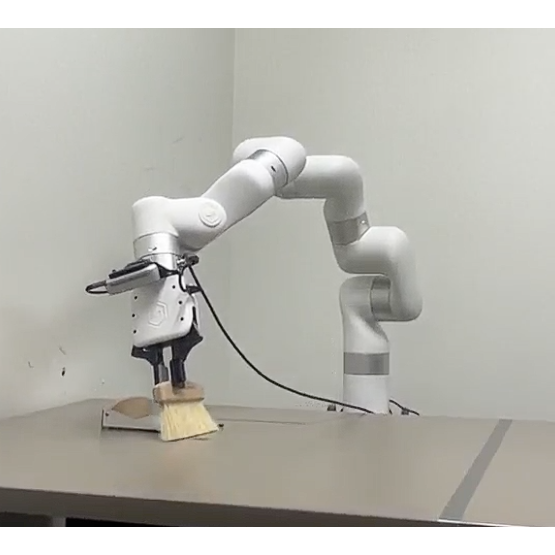
\includegraphics[width=\textwidth,trim={10pt 0 50pt 0},clip]{figures/examples/6.png}
          \end{minipage}\vspace{-2.5ex}
          \caption{\small \textbf{(Top)} Simulation tasks from Simpler~\cite{li24simpler}: {Close drawer}, {Move closer}, and {Pick Coke Can}. \textbf{(Bottom)} 
          Xarm7: {Stack Cubes}, {Duck in Bowl}, and {Sweep}.}
          \label{fig:xarm7}
        \end{minipage}
    \end{minipage}%
  \hfill
  \vspace{-0.5ex}
    \begin{minipage}{0.4\textwidth}
      \centering
      \begin{minipage}{0.45\linewidth}
        \centering
        \includegraphics[width=\textwidth]{figures/results/sim_res.pdf}
      \end{minipage}
      \hfill
      \begin{minipage}{0.49\linewidth}
        \centering
        \includegraphics[width=\textwidth]{figures/results/real_res.pdf}
      \end{minipage}
      \vspace{-2.5ex}
      \caption{\small Performance of models on simulated (left) and real (right) robotic tasks.}
      \label{fig:res}
    \end{minipage}\vspace{-1ex}
\end{wrapfigure}\vspace{-2.5ex}
\\
\noindent\textbf{\cib{5} ACT~\cite{zhao2023learningFB}:} ACT is a VLA model that uses ResNet~\cite{resnet} as the vision encoder and transformer-based
conditional variational autoencoder (CVAE)~\cite{sohn2015learning} that generates a sequence of actions. The original ACT 
was designed to process visual data and joint positions without additional language instructions. 
Similar to Octo~\cite{team2024octo}, ACT processes the images (multiple views if available, \eg original ACT uses 4 camera views) through a ResNet model, adds positional embeddings, and feeds them into a transformer-based CVAE-encoder (along with joint positions) to generate a sequence of actions (projected using MLP to chunks of absolute joint positions) through the CVAE-decoder.
\begin{comment}
For example, for Bimanual robots, the observation includes 4 RGB images (4 cameras), each at $480\times640$ resolution, and joint positions for two robot arms (7+7=14 positions in total).
The ResNet processes each image ($480\times640\times3$) and outputs feature maps of 4 images $\times$ $15\times20\times512$.
These feature maps are flattened ($1200\times512$), added to positional embeddings, and fed into the transformer encoder with additional joint position information.
The transformer decoder processes the encoder output through cross-attention to generate a sequence of actions ($k \times 512$ where $k$ is the number of action chunks). To generate the final actions, the output is down-projected with an MLP to $k \times 14$ dimensions, corresponding to the target joint positions for the next $k$ steps.
\end{comment}
Our implementation of ACT follows the original design, but changes are adopted to accommodate other embodiments, \eg change the number of views and action dimensions.%, 
\\
\BfParaUL{Preliminary Experiments: Robotic Models} 
We have conducted preliminary experiments to evaluate the performance of robotic models, \ie RT-1, RT-2, Octo, and ACT on simulated and real robotic tasks. 
For simulation, we used Simpler~\cite{li24simpler} benchmark for three tasks: \emph{Close the drawer}, \emph{Move closer}, and \emph{Pick the Coke Can} using Google robot embodiment, while for real experiments, we used Xarm7 robot for three tasks: \emph{Stack Cubes}, \emph{Duck in Bowl}, and \emph{Sweep} (see~\autoref{fig:xarm7}).
For the simulation tasks, models were fine-tuned (using single third-person view and language-conditioned control) using 50 episodes per task. Language instructions are not used for ACT. Five training runs were performed per model, where each run was trained for 20,000 iterations with a batch size of 512 and a learning rate of 1e-5 using AdamW optimizer. The evaluation was performed on 25 episodes per task over five runs with different random seeds.
Similar training and evaluation settings were used for the real robotic tasks, but with visual observations only and no language instructions to avoid any changes on the ACT model architecture. 
Task success is measured using a two-point scoring system. For \emph{Stack Cubes} (stacking two cubes) and \emph{Duck in a bowl} (placing duck in bowl), points are awarded for successful pick (1 point) and place (1 point) operations. For \emph{Sweep}, points are given for finding (1 point) and sweeping objects into the bin (1 point). The success rate is calculated as the average scores divided by the total points in all evaluation episodes.
The preliminary results are shown in~\autoref{fig:res}.
% \BfPara{Adoption and Constraints}
% At inference time, each model is required to run at the rate required for the robot (3-10~Hz). 
% While relatively small models, \eg ACT, Octo, RT-1 can run locally on some robots with such inference rate, larger models, \eg OpenVLA and RT-2 (7B+ parameters), are hosted on a cloud service and queried over the network. This can introduce latency and network reliability issues, which are critical for real-time robotic applications.
% Even when designing/training such models to generate chunks of actions at once, which can be executed over several time steps,
% robotic models require strict real-time performance for smooth operation. % unlike general LLM/VLMs which often operate without stringent timing constraints.
% This adds complexity to robotic models, \ie managing latency, network reliability, and data communication security aspects that are less critical in typical LLM/VLM applications.
% In terms of adversarial attacks, attacking a robot's availability through prompt injection or jailbreak attacks (\eg running prompts that take more than 15Hz) can have far more serious consequences than similar attacks on other LLM/VLM applications.
% Compromised availability (and/or functionality) of a robot from an attack can cause physical harm, property damage, or operational disruptions.
% The real-time and/or (network dependence) of these models adds vulnerabilities that can be exploited to disrupt availability, making it imperative to prioritize security and resilience against such attacks.


\BfParaUL{Preliminary Experiments: Attacking Robotic Models}
We have conducted two preliminary experiments
\begin{wrapfigure}{r}{0.25\textwidth}
\vspace{-2.5ex}
\centering
% \hspace{-2ex}
\begin{minipage}{0.25\textwidth}
\begin{minipage}{\textwidth}
\centering
\includegraphics[width=0.95\textwidth]{figures/results/visual_white_box.pdf}\vspace{-2ex}
\caption{\footnotesize Success rate of white-box attacks on robotic models using visual perturbations.}
\label{fig:visual_white_box}
\end{minipage}
% \hspace{-4ex}
\begin{minipage}{\textwidth}
  \centering
  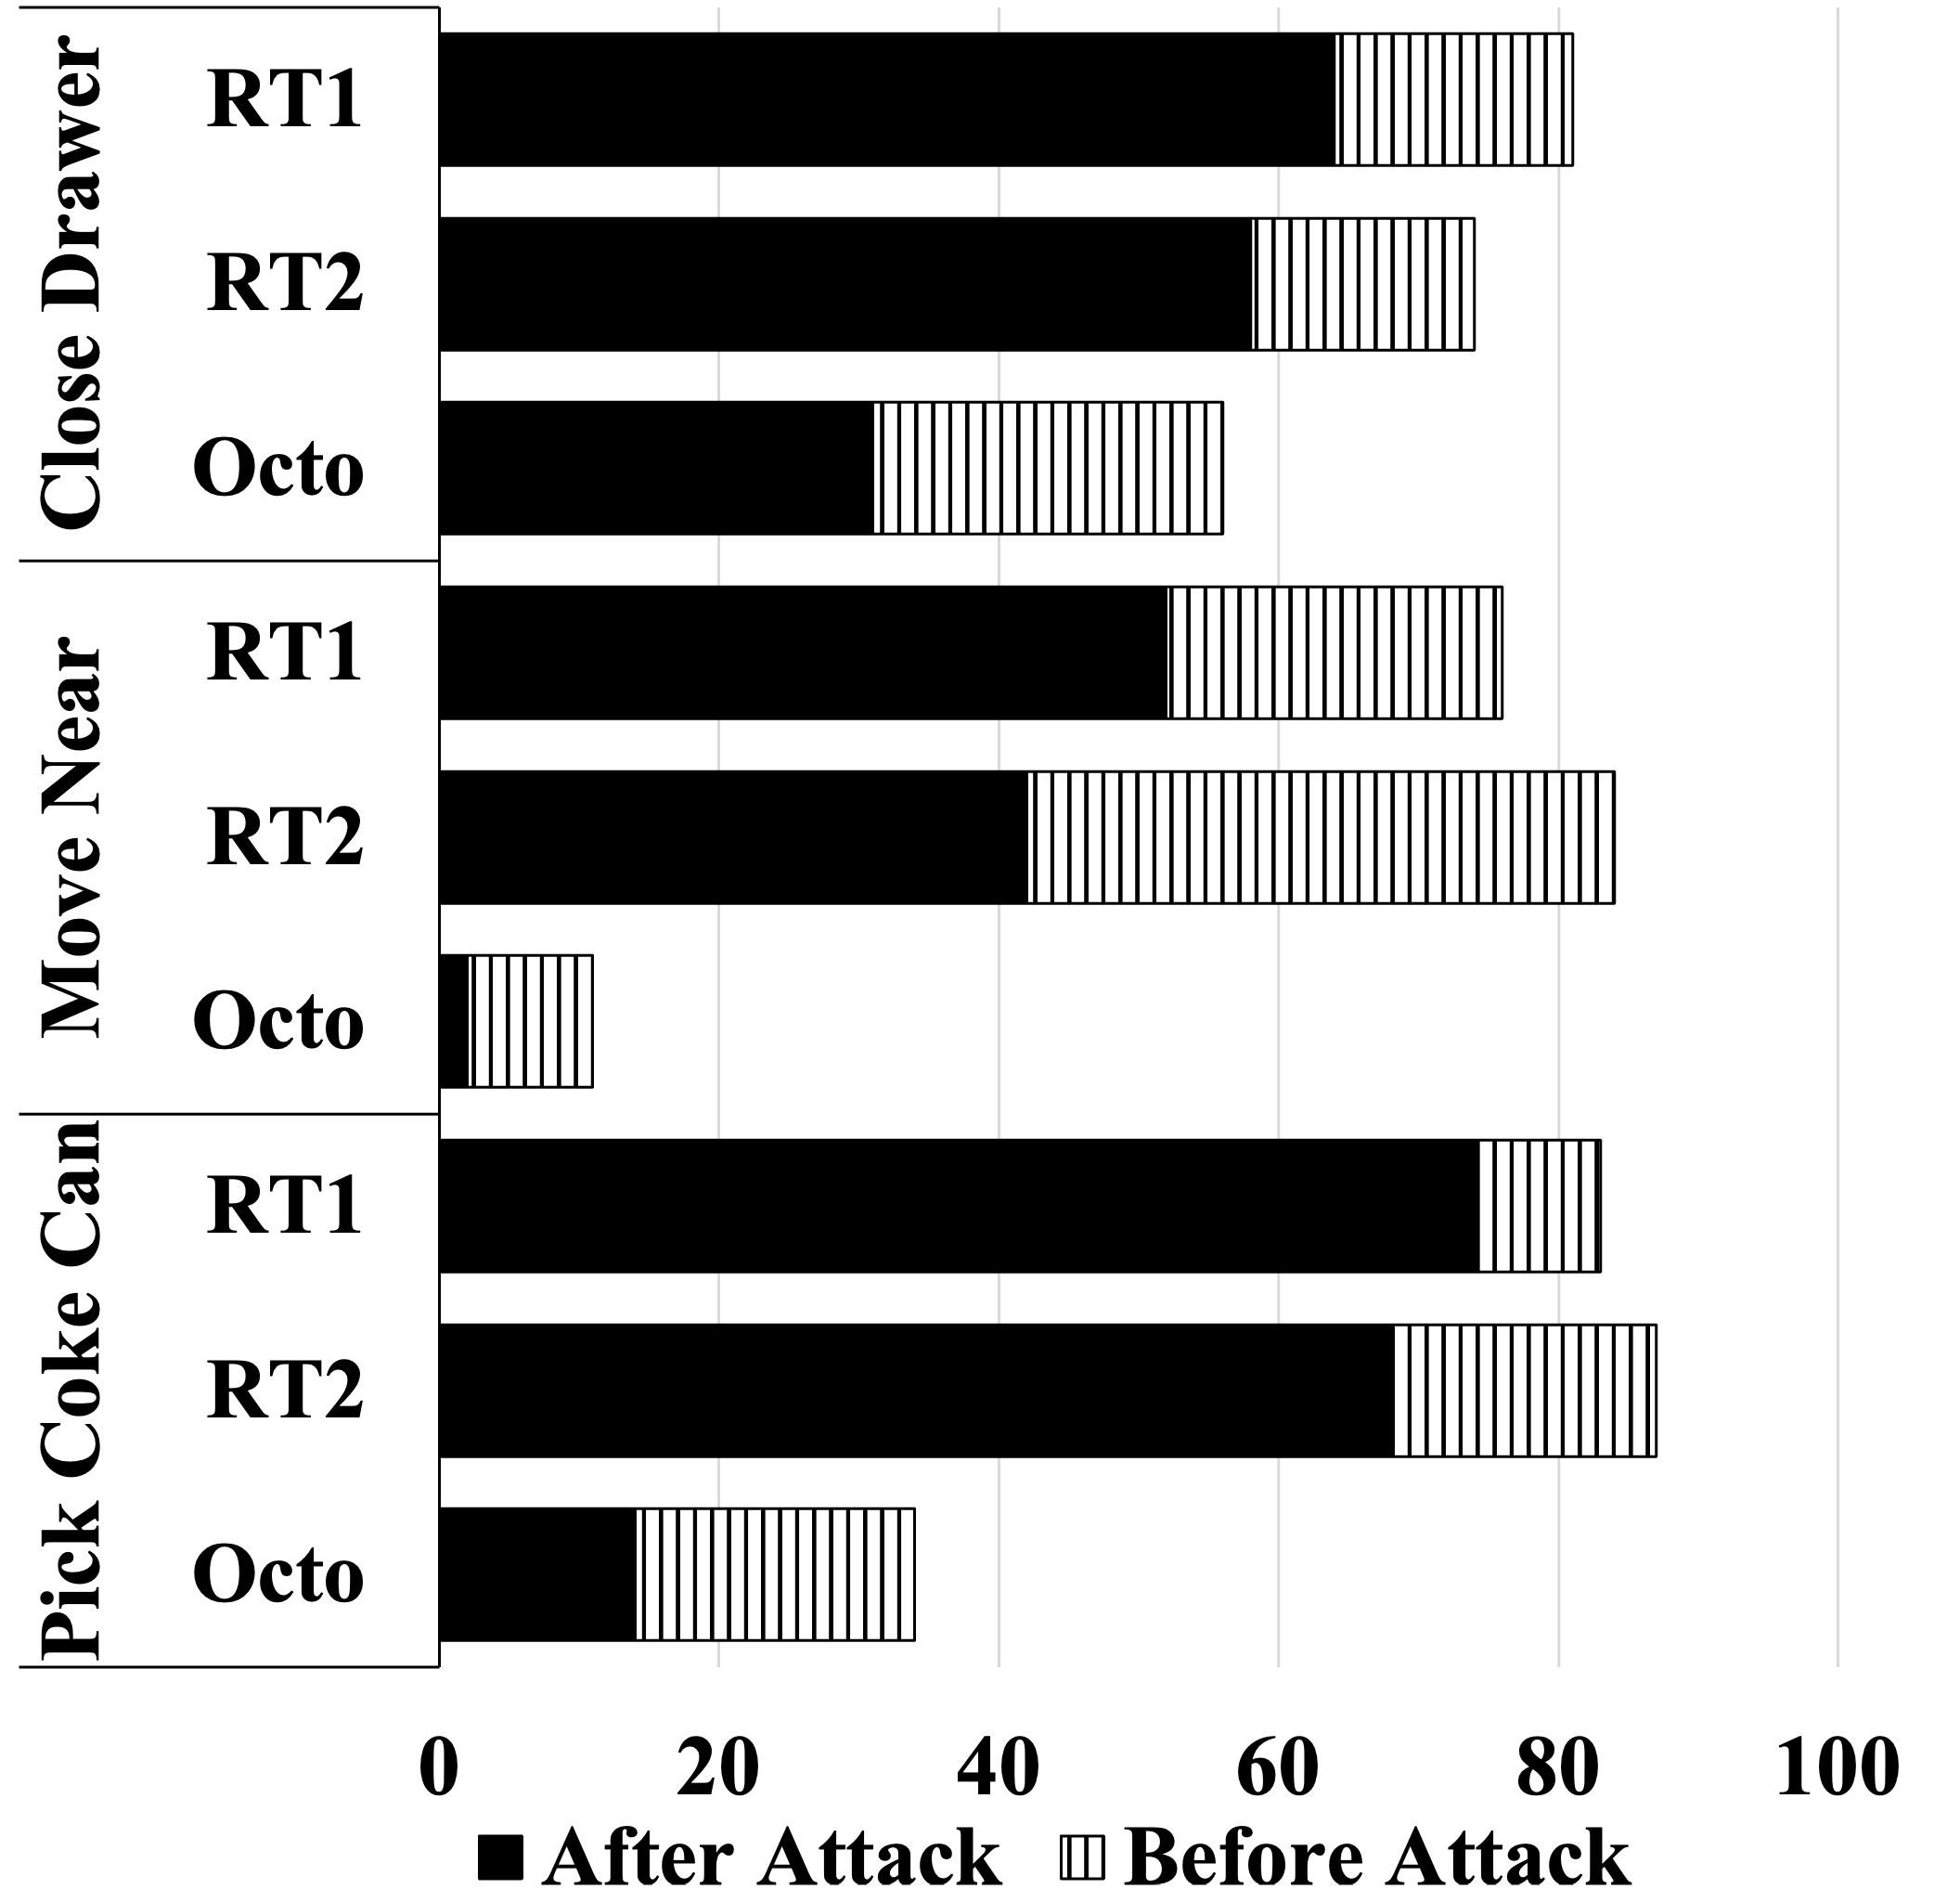
\includegraphics[width=0.95\textwidth]{figures/results/lang_black_box.pdf}\vspace{-2ex}
\caption{\footnotesize Task success rate of models before and after black-box token-based perturbations.}
  \label{fig:lang_black_box}
\end{minipage}
\end{minipage}
\vspace{-3ex}
\end{wrapfigure}
 to evaluate the effectiveness of adversarial attacks on models trained on Simpler~\cite{li24simpler} benchmark using three tasks. Both experiments were conducted on the same three tasks as in the preliminary experiments, and evaluated using 25 episodes repeated 5 times.
\textbf{Experiment 1:} We examined \emph{untargeted white-box} attacks using visual perturbations (\ie on image inputs) against robotic models. We implemented three baseline attack methods: PGD~\cite{madry2017towards}, FGSM~\cite{goodfellow2014explaining}, and CW~\cite{carlini2017towards}. This attack scenario assumes the attacker has complete access to the parameters of the model's visual encoder, \ie EfficientNet-B3 (RT-1), Vision Transformer (RT-2), and ResNet (Octo and ACT). Such an assumption is realistic since these robotic models typically incorporate open-source pre-trained visual encoders. %, making their architecture and parameters readily available to potential attackers.
We evaluated the success rate of the attacks by measuring the percentage of successful adversarial examples where the generated actions differ from the ground-truth actions with a threshold of 30\%. \autoref{fig:visual_white_box} shows the attack success rate on various models. 

\textbf{Experiment 2:} We examined \emph{black-box} attacks using token-based language perturbations (\ie on text inputs) against robotic models (except ACT as it does not support language instructions). We assume the attacker has no access to the model parameters and can only query the model. The attacker can manipulate the language instructions by deleting/replacing/adding tokens to the original instructions.
We adopted a similar attack approach to one used in SHIELD~\cite{abuhamad2025shield}, our previous work. %which focused on enhancing the robustness of code attribution models.
The attack perturbs 30\% of the tokens in the instructions with random tokens from the tokenizer vocabulary, and probes the model with a query limit of 500 queries. The attack terminates if the query limit is reached or if the model's output action differs from the ground-truth action by more than 30\%, in which case the attack is successful.
The results are shown
% {\vspace{-2.5ex}}
 in~\autoref{fig:lang_black_box}. %, where we observe that the success rate of the models drops significantly after the attack, indicating that even simple token-based perturbations can disrupt the model's performance.
These results demonstrate the potential vulnerabilities of robotic models to adversarial attacks.
% In these preliminary experiments we operationalized attack success as a 30\% action-token deviation. 
% In the full evaluation protocol described below, we use task success rate (TSR) under attack as the primary metric and use action deviation as a secondary physical-consequence metric.


















\subsection{T1: Full-Access Attacks on Robotic Foundation Models} \label{sec:t1}
Full-access (white-box) attacks exploit full access to the model's architecture and parameters.
White-box attacks provide deep insights into model vulnerabilities, enabling better understanding of its robustness.% and security of models, ensuring reliable and safe performance in real-world applications.
\\
\BfPara{Related Work} While the literature is rich in methods for white-box attacks against various models, the closest model families to generalist robot foundation models are VLMs.
Most evasion attacks against VLM \cite{schlarmann2023adversarial, bailey2023image,gao2024adversarial,wang2024stop,tan2024wolf} typically use gradient-based approaches, \eg PGD and CW, to generate/optimize perturbation for adversarial samples.
Recent work has begun to move beyond static, single-frame formulations toward trajectory-level redirection and architecture-specific attacks designed to flow-matching robot policies~\cite{puthumanaillam2026trajectory,tae2026drift}.
A recent study \cite{fu2023misusing} shows that seemingly harmless images with trojan-like characteristics can manipulate VLMs to call attacker-specific third-party tools or external APIs. 
Gao \etal \cite{gao2024inducing} introduce verbose images, creating imperceptible perturbations to make VLMs generate longer output sentences. Such an attack raises energy consumption and latency, which can have serious consequences in robotics.
\ul{In this task, we propose new attack family, Action-Bin Boundary Perturbation (ABBP), and investigate the cross-modal behavior in evasion and poisoning scenarios against robotics models.}

\subsubsection{T1-1: White-Box Action-Space Attacks} \label{sec:t1_1}

\BfPara{Proposed Attack} 
We propose ABBP, a gradient-based white-box attack designed to exploit the uniform 256-bin discretization of the VLA action space. Because adjacent bins encode physically close but discretely different control signals, ABBP optimizes perturbations to drive predicted action tokens across bin boundaries.
Let $\mathcal{C}\subseteq\{1,\dots,d\}$ denote the $d$-dimensional continuous action, each uniformly quantized into $B{=}256$ bins, leaving $\{1,\dots,d\}\setminus\mathcal{C}$ for the discrete dimensions ({\eg} RT-1's arm/base/terminate mode). For $j\in\mathcal{C}$ the model $\mathcal{F}$ outputs logits $\bm{z}_j(\bm{\{x\}}, \bm{\{t\}})\in\mathbb{R}^{B}$, and the decoded bin and action are 
\vspace{-1ex}\begin{equation} 
  \small b_j=\argmax_{c\in\{0,\dots,B-1\}} z_{j,c}(\bm{\{x\}}, \bm{\{t\}}), \qquad \hat a_j=l_j+\bigl(b_j+\tfrac{1}{2}\bigr)\Delta_j, \qquad \Delta_j=\frac{u_j-l_j}{B}, 
  \label{eq:abbp-quant} 
\vspace{-1.5ex}
\end{equation} 
with $[l_j,u_j]$ the range of dimension $j$ and $\Delta_j$ the bin width. We set $\Delta_j{=}0$ for $j\notin\mathcal{C}$ and write $\hat{\bm{a}}\in\mathbb{R}^{d}$ and $\bm{\Delta}=[\Delta_1,\dots,\Delta_d]^{\top}$ for the decoded action and the bin-width vector. Uniform binning fixes $\Delta_j$ independently of the local sensitivity of the task, so a single-bin logit flip always carries a bounded but non-zero physical displacement. 
{\bf \emph{Kinematic map:}} Let $\mathcal{J}\subseteq\mathcal{C}$ index the dimensions driving the arm, excluding the gripper aperture and the base dimensions, so $|\mathcal{J}|{=}6$ in end-effector action spaces and $|\mathcal{J}|{=}n$ for an $n$-joint arm in joint space. For a joint configuration $\bm{\theta}$ and an action increment $\bm{u}\in\mathbb{R}^{d}$, the end-effector displacement over one control period $\tau$ is $G(\bm{\theta})\bm{u}\in\mathbb{R}^{6}$, where $G(\bm{\theta})\in\mathbb{R}^{6\times d}$ vanishes on columns outside $\mathcal{J}$ and restricts on $\mathcal{J}$ to $I_{6}$ for end-effector position spaces ({\eg} RT-1, RT-2, OpenVLA, and most of \autoref{tab:multi_dataset}), $\tau I_{6}$ for end-effector velocity spaces ({\eg} ConqHose, FMB), and the manipulator Jacobian $J(\bm{\theta})$ for joint-space actions ({\eg} ACT, RoboSet, SPOC), the last being the first-order approximation valid for the small increments considered here. These cover the action-space families of \autoref{tab:multi_dataset}. Because a twist mixes length and angle units, we measure displacement as $\|W G(\bm{\theta})\bm{u}\|_{2}$ with $W=\mathrm{diag}(1,1,1,\ell,\ell,\ell)$ and $\ell$ a characteristic lever arm of the embodiment.



ABBP exploits this structure in two stages.
\cib{1} \emph{Target selection:} ABBP selects a coordinated bin-shift vector $\bm{s}\in\mathbb{Z}^{d}$ maximizing end-effector displacement under budget and kinematic-feasibility constraints,
\vspace{-1ex}\begin{equation}
  \small
\bm{s}^{*}=\argmax_{\substack{\bm{s}\in\mathbb{Z}^{d},\; s_j=0\;\forall j\notin\mathcal{J}}}
\bigl\|W G(\bm{\theta})\,(\bm{s}\odot\bm{\Delta})\bigr\|_{2}
\;\;\text{s.t.}\;\;
\|\bm{s}\|_{1}\le\beta,\;\;
\|\bm{s}\|_{\infty}\le\sigma,\;\;
0\le b_j+s_j\le B-1,
\label{eq:abbp-shift}
\vspace{-1.5ex}\end{equation}
subject to $\hat{\bm{a}}+\bm{s}\odot\bm{\Delta}\in\mathcal{A}(\bm{\theta})$. Here $\odot$ is the
elementwise product, and $\beta$ and $\sigma$ are the total and per-dimension bin-shift budgets with
$\sigma<\beta$. The feasible set $\mathcal{A}(\bm{\theta})$ holds every action $\bm{a}$ obeying the
per-step velocity bound $\|\bm{a}-\hat{\bm{a}}\|_{\infty}\le\dot a_{\max}\tau$ for a per-dimension
action-rate limit $\dot a_{\max}$, and reaching a configuration $\psi(\bm{\theta},\bm{a})$ inside the
joint limits $\mathcal{L}$ and the reachable workspace $\mathcal{W}$ after one control period $\tau$.
The objective is convex in $\bm{s}$, so $\beta$ alone would spend the budget on the single
highest-gain dimension, while $\sigma$ spreads the shift across several degrees of freedom, and the
bin bounds keep $b_j+s_j^{*}$ decodable without post-hoc clipping.
\cib{2} \emph{Perturbation synthesis:} With $b_j^{*}=b_j+s_j^{*}$, ABBP solves a margin objective over the visual input (expandable to textual input as well),
\vspace{-3ex}\begin{equation}
  \small
\min_{\bm{\delta}}\;\sum_{j=1}^{d} w_j
\Bigl[\max_{c\neq b_j^{*}} z_{j,c}(\bm{x}+\bm{\delta},\bm{t})-z_{j,b_j^{*}}(\bm{x}+\bm{\delta},\bm{t})+\kappa\Bigr]_{+}
\quad\text{s.t.}\quad
\|\bm{\delta}\|_{\infty}\le\epsilon,\;\;\bm{x}+\bm{\delta}\in[0,1]^{N},
\label{eq:abbp-obj}
\vspace{-1.5ex}\end{equation}
where $\bm{\delta}$ is the additive image perturbation, $\epsilon$ its $\ell_{\infty}$ budget, and $N$ the number of pixel values in $\bm{x}$, with $[\cdot]_{+}=\max(\cdot,0)$, confidence margin $\kappa$, and box constraint in raw pixel space before encoder normalization. The weights are $w_j=\|(WG(\bm{\theta}))_{:,j}\|_{2}\Delta_j$ for $j\in\mathcal{J}$, so the optimizer allocates perturbation budget to the dimensions with the largest physical effect per bin, and $w_j=\lambda$ for $j\notin\mathcal{J}$. 
\autoref{eq:abbp-obj} treats the $d$ logit vectors as conditionally independent, which holds for parallel readout heads ({\eg} RT-1, Octo). For autoregressive action decoders ({\eg} RT-2, OpenVLA), the action tokens form a sequence and $\bm{z}_j$ depends on the preceding tokens, so we evaluate each margin under teacher forcing on the target prefix $b^{*}_{<j}$. We solve \autoref{eq:abbp-obj} by projected gradient descent with step $\alpha$ over $T$ iterations. Setting $w_j{=}1$ for $j\in\mathcal{J}$ and $\sigma{=}1$ while retaining $\mathcal{A}(\bm{\theta})$ yields a discretization-agnostic variant, isolating the contribution of the physical-effect weighting in an ablation.


\BfPara{ABBP in Poisoning Scenarios} The two-stage design of ABBP extends from \emph{evasion} to training-time \emph{poisoning} attacks (see \autoref{table:attacks_models}). 
In evasion, ABBP perturbs the input under budget $\epsilon$. In poisoning, the attacker applies the
target selection $\bm{s}^{*}$ (\autoref{eq:abbp-shift}) and the margin objective
(\autoref{eq:abbp-obj}) to training data, action labels, or gradient updates, and we reinterpret the
attack budget as the poison rate, \ie the fraction of corrupted samples or updates.
For example,
because VLA action labels are bin indices, \emph{data poisoning} and \emph{label flipping} reduce to
setting $b_j \rightarrow b_j+s^{*}_{j}$ on the dimensions \autoref{eq:abbp-shift} selects, where a
shift of at most $\sigma$ bins encodes a physically adjacent action and evades label inspection. 
\emph{Backdoor poisoning} pairs a visual or textual trigger with labels fixed at $b_j^{*}=b_j+s_j^{*}$, so the trigger induces a kinematically feasible displacement of maximal magnitude at inference, while \emph{clean-label} and \emph{targeted} poisoning variants keep labels intact and instead
perturb the observation so the model binds a context to the shifted mapping $b^{*}_{j}$. 
\emph{Subpopulation poisoning} concentrates corrupted samples on configurations with high kinematic
gain $\|(WG(\bm{\theta}))_{:,j}\|_{2}$, limiting degradation on clean data outside the target
subpopulation.
\emph{Model poisoning}, \emph{model replacement}, and \emph{model boosting} assume gradient- or model-channel access, \eg federated fine-tuning or fine-tuning-as-a-service, and use the ABBP margin as an auxiliary training loss, biasing logits near bin boundaries while clean task success stays high. \emph{Functional attacks} follow the same pattern, poisoning the learned policy toward systematic violation of a behavioral property such as the per-step velocity bound $\|\bm{a}-\hat{\bm{a}}\|_{\infty}\le\dot a_{\max}\tau$. 



\BfPara{ABBP Evaluation} We evaluate ABBP under the shared protocol (\autoref{eq:abbp-gate}) with $\gamma{=}0.7$ and baselines PGD, FGSM, and CW. We calibrate $(\sigma,\rho)$ against the reachability bound $\rho\le H\sqrt{|\mathcal{J}|}\,\sigma\max_{j\in\mathcal{J}}\|(WG(\bm{\theta}))_{:,j}\|_{2}\Delta_{j}$ implied by \autoref{eq:abbp-quant} and \autoref{eq:abbp-shift}, so the target remains reachable before any experiment runs. We also report the discretization-agnostic ablation ($w_j{=}1$, $\sigma{=}1$) to isolate the contribution of the physical-effect weighting.







\subsubsection{T1-2: Multimodal White-Box Action-Space Attacks}  \label{sec:t1_2}
This task aims to examine the security and defense strategies derived from the targeting of one or more modalities used by robots. 
Although much progress has been made in designing adversarial attacks in individual modalities (\eg vision or language), the interaction between modalities remains less explored. Existing attackers, even with multimodal systems, generally treat the perturbations of different modalities separately and design them independently. 
However, this results in less interactive relations between the perturbed multimodal inputs and can be easily recognized by security alignment methods (\ie methods
to align the model behavior with expected values and intentions). 
In addition, along with visual and textual instructions, other modalities can be incorporated in the training of generalist robots. Some of these modalities can be sensory information, tabular environment data, or supplementary interpretation maps (\ie maps that indicate the region of importance in recent outputs). 

To date, emerging foundation models in robotics focus mainly on visual and textual instruction. With the current trend of democratization of data and models, we expect and plan to explore more modalities as they emerge as common information used by robots.
We note that incorporating additional modalities into the system provides attackers with more physical avenues to launch attacks.
\ul{Our aim is to explore novel ways to reveal vulnerabilities by crafting ``\textit{tightly-multimodal}'' adversarial examples that simultaneously perturb visual and textual input with strong connections.} 
We will target the vision-language coupling mechanism specific to each model, namely FiLM in RT-1~\cite{rt-1}, a projection MLP in OpenVLA~\cite{kim2024openvla}, and cross-attention in Octo~\cite{team2024octo}, and formulate a model-specific co-perturbation objective at each mechanism so the visual and textual perturbations co-reinforce at the grounding layer. To test coupling on a further language-conditioned policy, we include OpenVLA-OFT or a language-conditioned Octo variant, and we exclude vision-only policies such as ACT from this multimodal scope. We present T2 as a scale-up track in Years~3 and~4 that builds on the attack baselines established in T1.
This includes studying the interactions and dependencies between modalities to create more effective cross-modal attacks that can evade current defenses. For example, Multi-key strategies~\cite{walmer2022dual} could be used to improve the connections between multimodal perturbations and co-control the attack.
Multimodal prompt injection attacks simultaneously alter both textual and visual modalities, injecting adversarial semantics into multiple modalities to enhance the possibility of overcoming alignment methods.
Recent studies \cite{qi2024visual,shayegani2023jailbreak} show that adversarial perturbations of visual and textual modalities can jointly succeed in creating malicious injections.
Recent work has begun to explore physical attention-hijacking and patch attacks that target the vision-language grounding of robot policies, which we will build on and compare against~\cite{zhang2026structure,yin2026vlaguard}.
By understanding and leveraging these interactions, we aim to develop more robust defense mechanisms that can protect against sophisticated multimodal adversarial attacks. We will also assess robustness techniques such as CleanCLIP~\cite{bansal2023cleanclip}, which retrains multimodal representations to reduce cross-modal misalignment, as a complementary defense against these attacks.
\ul{In this task, variations of ABBP attacks will be explored and evaluated.}

\BfPara{ABBP over Language Instructions}
The two-stage design of ABBP extends from the visual input to the language instruction $\bm{t}$ with no change to the action-space machinery, because only perturbation synthesis touches the input domain.
Target selection (\autoref{eq:abbp-shift}) operates entirely in action and kinematic space, so it is modality-agnostic and transfers verbatim; the selected shift $\bm{s}^{*}$ and target bins $b_j^{*}=b_j+s_j^{*}$ are unchanged.
What changes is the synthesis step (\autoref{eq:abbp-obj}): instead of perturbing the image, we perturb the instruction and solve the same weighted hinge margin over the logits, now driven by $\bm{t}$,
\vspace{-1ex}\begin{equation}
  \small
\min_{\bm{t}'}\;\sum_{j=1}^{d} w_j
\Bigl[\max_{c\neq b_j^{*}} z_{j,c}(\bm{x},\bm{t}')-z_{j,b_j^{*}}(\bm{x},\bm{t}')+\kappa\Bigr]_{+}
\quad\text{s.t.}\quad
\mathcal{C}_{\mathrm{text}}(\bm{t},\bm{t}')\le\epsilon_t,
\label{eq:abbp-obj-text}
\vspace{-1.5ex}\end{equation}
where $\bm{t}'$ is the perturbed instruction and the weights $w_j=\|(WG(\bm{\theta}))_{:,j}\|_{2}\Delta_j$ and margin $\kappa$ are exactly those of \autoref{eq:abbp-obj}.
Because the input is a discrete token sequence, we replace the projected-gradient solver of \autoref{eq:abbp-obj} with a first-order token-substitution search in the embedding space of the instruction encoder, followed by nearest-token projection; the gradient of the margin with respect to each token embedding identifies the highest-impact replacements.
The constraint $\mathcal{C}_{\mathrm{text}}$ must play the role that the $\ell_{\infty}$ ball and pixel box play for vision, and it carries two requirements.
The first is a bounded edit budget $d_{\mathrm{edit}}(\bm{t},\bm{t}')\le k$ together with an embedding-similarity floor, so the perturbation stays imperceptible in the same sense that $\epsilon$ bounds the pixel change.
The second is semantic equivalence: without it, editing the instruction degenerates into changing the task rather than attacking it, and the clean reference trajectory in \autoref{eq:abbp-gate} no longer isolates the effect of the attack.
We therefore restrict $\bm{t}'$ to meaning-preserving edits, namely synonym substitution, paraphrase, reordering, misspelling, and appended adversarial suffixes, and we enforce this with a similarity threshold under a reference sentence encoder.
The poisoning constructions of \autoref{sec:t1_1} extend to the textual channel unchanged, since label flipping and backdoor poisoning already admit a textual trigger paired with the shifted labels $b_j^{*}$.

\BfPara{ABBP over Joint Visual and Language Input}
We then formulate the tightly-multimodal attack as a joint optimization over both modalities.
Let $\bm{\delta}_x$ denote the visual perturbation of \autoref{eq:abbp-obj} and $\bm{t}'$ the perturbed instruction of \autoref{eq:abbp-obj-text}. The joint objective couples the shared action-margin loss with a grounding term that forces the two perturbations to co-reinforce at the vision-language fusion layer,
\vspace{-1ex}\begin{equation}
  \small
\min_{\bm{\delta}_x,\,\bm{t}'}\;\sum_{j=1}^{d} w_j
\Bigl[\max_{c\neq b_j^{*}} z_{j,c}(\bm{x}+\bm{\delta}_x,\bm{t}')-z_{j,b_j^{*}}(\bm{x}+\bm{\delta}_x,\bm{t}')+\kappa\Bigr]_{+}
\;-\;\lambda_c\,\bigl\|\Psi(\bm{x}+\bm{\delta}_x,\bm{t}')-\Psi(\bm{x},\bm{t})\bigr\|_{2}
\label{eq:abbp-obj-joint}
\vspace{-1.5ex}\end{equation}
subject to $\|\bm{\delta}_x\|_{\infty}\le\epsilon_x$, $\bm{x}+\bm{\delta}_x\in[0,1]^{N}$, and $\mathcal{C}_{\mathrm{text}}(\bm{t},\bm{t}')\le\epsilon_t$.
Here $\Psi$ is the model-specific coupling mechanism named above, \eg FiLM in RT-1, the projection MLP in OpenVLA, and cross-attention in Octo, and $\lambda_c$ weights the coupling term so the visual and textual perturbations align at grounding rather than act independently.
Because one modality is continuous and the other discrete, we solve \autoref{eq:abbp-obj-joint} by alternating optimization: a projected-gradient step on $\bm{\delta}_x$ reuses the solver of \autoref{eq:abbp-obj} unchanged, and a token-substitution step on $\bm{t}'$ reuses the textual search of \autoref{eq:abbp-obj-text}, iterating until the margin converges.
The joint formulation also exposes the budget split $(\epsilon_x,\epsilon_t)$ as an experimental variable; we will report attack success across this split to measure how much textual budget substitutes for pixel budget in each model, which directly quantifies the cross-modal interaction that single-modality attacks cannot capture.
The evaluation protocol of \autoref{eq:metric-stack} carries over without modification because it is computed from end-effector poses and decoded bins; we add only text-side imperceptibility metrics, specifically edit distance and embedding similarity, alongside the $\ell_{\infty}$ pixel budget so the textual perturbation is held to the same stealth standard as the visual one.

 \subsubsection{Evaluation Protocol}

All attack families are evaluated under one protocol with
three metrics computed from a single episode. 
Let $\mathcal{E}$ be the evaluation episodes of a task ($|\mathcal{E}|{=}25$) and $\mathcal{I}$ the independent seeds ($|\mathcal{I}|{=}10$). Each
episode $e\in\mathcal{E}$ is run twice from an initial state, once on clean observations and once with $\mathcal{M}$ active at budget $\epsilon$, re-optimized at every step. 
For inference-time attacks, $\epsilon$ is the $\ell_{\infty}$ bound of \autoref{eq:abbp-obj}; for training-time attacks it is the poison rate. 
In both cases $\epsilon$ is drawn from a fixed geometric grid $E$ capped at $\epsilon_{\max}$. A run returns a task score $v_{\mathcal{M}}(e,\epsilon)\in[0,1]$ under the two-point scoring of \autoref{sec:t0}, the end-effector poses $(\bm{p}_{k},R_{k})$ and $(\bm{p}'_{k},R'_{k})$ for $k=0,\dots,H$ from forward kinematics, and the decoded bins $b_{j,k}$ and $b'_{j,k}$ of \autoref{eq:abbp-quant}.
We write $v_{0}(e)=v_{\mathcal{M}}(e,0)$ and $\mathcal{E}_{0}=\{e\in\mathcal{E}:v_{0}(e)=1\}$ for the episodes the undefended policy completes. We fix $H$ at one quarter of the median episode of the embodiment. We measure the following metrics.

\cib{1} \textbf{Physical consequence.} Comparing the two pose sequences,
\vspace{-1ex}\begin{equation}
  \small
\bm{e}_{k}=\begin{bmatrix}\bm{p}'_{k}-\bm{p}_{k}\\[2pt] rv\bigl(R_{k}^{\top}R'_{k}\bigr)\end{bmatrix},
\qquad
D^{e}_{\mathcal{M}}(H)=\bigl\|W\bm{e}_{H}\bigr\|_{2},
\qquad
\bar{D}^{e}_{\mathcal{M}}(H)=\max_{0\le k\le H}\bigl\|W\bm{e}_{k}\bigr\|_{2},
\label{eq:abbp-gate}
\vspace{-1.5ex}\end{equation}
where $rv$ is the rotation-vector map of the relative rotation and $W=\mathrm{diag}(1,1,1, \ell,\ell,\ell)$ weights rotational displacement by the characteristic lever arm $\ell$ of the embodiment, so that $D$ and $\bar{D}$ carry units of length. $D^{e}_{\mathcal{M}}(H)$ is the terminal deviation, written $D_{\mathcal{M}}(H)$ when the episode is implicit; the peak deviation $\bar{D}^{e}_{\mathcal{M}}(H)$ is also reported. The threshold $\rho$ is calibrated per task (\ie based on the gripper-aperture clearance and the size of manipulated object, \eg $\rho{=}5$\,cm in preliminary tasks).
\cib{2} \textbf{Task and attack success.} From the same runs,
\vspace{-1ex}\begin{equation}
  \small
\mathrm{TSR}_{\mathcal{M}}(\epsilon)=\frac{1}{|\mathcal{E}|}\sum_{e\in\mathcal{E}}
v_{\mathcal{M}}(e,\epsilon),
\quad
\mathrm{ASR}^{\mathrm{task}}_{\mathcal{M}}(\epsilon)=\frac{1}{|\mathcal{E}_{0}|}
\sum_{e\in\mathcal{E}_{0}}\mathbb{1}\bigl[v_{\mathcal{M}}(e,\epsilon)<1\bigr],
\quad
\mathrm{ASR}^{\mathrm{phys}}_{\mathcal{M}}(\epsilon)=\frac{1}{|\mathcal{E}|}
\sum_{e\in\mathcal{E}}\mathbb{1}\bigl[D^{e}_{\mathcal{M}}(H)\ge\rho\bigr],
\label{eq:metric-stack}
\vspace{-1.5ex}\end{equation}
and, at the token level,
$\mathrm{ASR}^{\mathrm{tok}}_{\mathcal{M}}(\epsilon)=(|\mathcal{E}|H)^{-1}\sum_{e,k}
\mathbb{1}[\exists j\in\mathcal{J}:b'_{j,k}\neq b_{j,k}]$ for untargeted attacks, replaced by
$\mathbb{1}[\exists j:b'_{j,k}{=}b^{*}_{j,k}]$ and $\mathbb{1}[b'_{j,k}{=}b^{*}_{j,k}\,\forall
j\in\mathcal{J}]$ for the targeted \textit{Contain} and \textit{Exactmatch} criteria
\cite{lu2024test,luo2024image}, with $b^{*}_{j}$ the target bin of \autoref{eq:abbp-shift}.
Conditioning $\mathrm{ASR}^{\mathrm{task}}$ on $\mathcal{E}_{0}$ prevents baseline policy
failures from inflating it. 
%A token flip is necessary but not sufficient for displacement,
% which is necessary but not sufficient for task failure, so we expect
% $\mathrm{ASR}^{\mathrm{task}}\le\mathrm{ASR}^{\mathrm{phys}}\le\mathrm{ASR}^{\mathrm{tok}}$. 

\cib{3} \textbf{Attack cost and comparison.} For an effect $\Phi$ and threshold
$\rho_{\Phi}$,
\vspace{-1ex}\begin{equation}
  \small
\epsilon^{*}_{\mathcal{M}}(\Phi,\rho_{\Phi})=\min\bigl\{\epsilon\in E:\;
\widehat{\mathbb{E}}\bigl[\Phi_{\mathcal{M}}(\epsilon)\bigr]\ge\rho_{\Phi}\bigr\},
\qquad
\hat{\gamma}^{\,i}_{\mathcal{M}_{b}}=
\frac{\epsilon^{*,i}_{\mathcal{M}_{b}}(\Phi,\rho_{\Phi})}
{\min_{\mathcal{M}\in\{\mathcal{M}_{1},\dots,\mathcal{M}_{m}\}}
\epsilon^{*,i}_{\mathcal{M}}(\Phi,\rho_{\Phi})},
\label{eq:budget-operator}
\vspace{-1.5ex}\end{equation}
with $\epsilon^{*}_{\mathcal{M}}=\epsilon_{\max}$ when no grid point reaches $\rho_{\Phi}$, the expectation taken over $\mathcal{E}$, and $\epsilon^{*,i}$ the value estimated on seed $i\in\mathcal{I}$. 
% We instantiate $\Phi$ three ways: the task instantiation $\epsilon^{*}_{\mathrm{TSR}}=\epsilon^{*}\bigl(1-\mathrm{TSR}_{\mathcal{M}}(\epsilon)/ \mathrm{TSR}_{\mathcal{M}}(0),\,\rho_{\mathrm{TSR}}\bigr)$ with $\rho_{\mathrm{TSR}}{=}0.5$, the budget that halves task success, which is our primary metric; the physical instantiation $\epsilon^{*}_{\mathrm{phys}}=\epsilon^{*}(D_{\mathcal{M}}(H),\rho)$, which resolves attacks whose displacement has not yet crossed a task boundary; and the token instantiation $\epsilon^{*}_{\mathrm{tok}}=\epsilon^{*}(\mathrm{ASR}^{\mathrm{tok}}_{\mathcal{M}},0.5)$, which requires forward passes only. 
We define $\Phi$ in three forms, based on the task success, the physical displacement, and the action-token-level attack success. For the task form, 
$\epsilon^{*}_{\mathrm{TSR}}=\epsilon^{*}(1-\mathrm{TSR}_{\mathcal{M}}(\epsilon)/
\mathrm{TSR}_{\mathcal{M}}(0),\,0.5)$ is the budget halving task success. 
The physical form $\epsilon^{*}_{\mathrm{phys}}=\epsilon^{*}(D_{\mathcal{M}}(H),
\rho)$ resolves displacement below task failure. The token form
$\epsilon^{*}_{\mathrm{tok}}=\epsilon^{*}(\mathrm{ASR}^{\mathrm{tok}}_{\mathcal{M}},
0.5)$ needs forward passes only.
We report $\mathcal{M}_{b}$ as a distinct vulnerability over $\mathcal{M}_{1},\dots,\mathcal{M}_{m}$ when the median of $\hat{\gamma}^{\,i}_{ \mathcal{M}_{b}}$ over $\mathcal{I}$ satisfies $\hat{\gamma}_{\mathcal{M}_{b}}\le\gamma$ on $\epsilon^{*}_{\mathrm{TSR}}$ for at least two of three tasks. Weaker adversarial knowledge relaxes $\gamma$ ($\gamma{=}0.7$ in white-box, $\gamma_{g}{=}0.8$ in gray-box, $\gamma_{b}{=}0.9$ in black-box).

\subsubsection{Deliverables} \label{sec:t1_deliverables}
T1 delivers four results. \cib{1} Open-source reference implementations of ABBP in its visual, textual, and joint variants, covering evasion and the poisoning classes of \autoref{table:attacks_models}, with the PGD, FGSM, and CW baselines under the shared protocol. \cib{2} A per-model and per-task vulnerability benchmark reporting $\mathrm{TSR}_{\mathcal{M}}$, $\mathrm{ASR}^{\mathrm{task}}$, $\mathrm{ASR}^{\mathrm{phys}}$, $\mathrm{ASR}^{\mathrm{tok}}$, and $\epsilon^{*}(\rho)$ on the models and datasets of \autoref{tab:multi_dataset}, including the reachability calibration of $(\sigma,\rho)$. \cib{3} A budget-split study over $(\epsilon_x,\epsilon_t)$ quantifying how textual budget substitutes for pixel budget per model, identifying which vision-language coupling (FiLM, projection MLP, cross-attention) is most exploitable. \cib{4} An ablation isolating the physical-effect weighting ($w_j{=}1$, $\sigma{=}1$) and the poisoning rate, establishing which stages of the two-stage design drive attack success.


\begin{comment}
\subsubsection{Evaluation Plan and Deliverables} \label{sec:t2_evaluation}

We will benchmark various multimodal attacks, measuring their effectiveness across multiple robot embodiments and tasks. As in T1, our primary metric is task success rate (TSR) under attack, with the 30\% action-token deviation retained as a secondary proxy.
In addition to attack evaluation metrics, such as Attack Success Rate, 
\textit{Contain} \cite{lu2024test}, \textit{Exactmatch} \cite{luo2024image,lu2024test}, transferability, and imperceptibility, we will use cross-modal benign-adversarial shifting to evaluate the impact of different modality in achieving adversarial objective.
For example, assess whether the attack can succeed or change behavior when an input to a successful multimodal attack (\ie $\mathcal{F}(\mathcal{M}(\bm{x},\bm{t}))\rightarrow\bm{a}_{out}'$) is mutated, \eg $\{\mathcal{M}(\bm{x},\bm{t})\} \rightarrow\{\mathcal{M}(\bm{x}),\bm{t}\}$ or $\{\bm{x},\mathcal{M}(\bm{t})\}$.
The mutation process can be adjusted to alter the extent of shifts required to facilitate behavior change.
As in T1, we also report maximum end-effector action displacement and safety-zone and force-threshold violation rate, each as mean~$\pm$~std over at least ten runs with significance assessed by Welch's $t$-test, and we contribute the multimodal attacks to the full cross-model transferability matrix.
We will align this protocol with recent physically-grounded evaluation practice for robot policies~\cite{sun2026maniparena}.
Deliverables include: \cib{1} a comprehensive framework for multimodal attacks/defenses against robotic foundation models, analyzing how vulnerabilities propagate across modalities, \cib{2} open-source implementations of developed multimodal attacks, defenses, and benchmarks, and \cib{3} academic publications/reports/labs on findings and methodologies.

 \end{comment}

\subsection{T2: Limited-Access Attacks on Robotic Foundation Models} \label{sec:t2}

\subsubsection{T2-1: Gray-box Attacks}\label{sec:t2_1}
Gray-box attacks exploit partial knowledge of the victim model, \eg the architecture and training data, to expose vulnerabilities under moderate adversarial capabilities. For example, existing gray-box attacks against VLMs use open-source vision or language encoders as surrogates to launch the attack.
Attacks include \emph{prompt injection} and \emph{jailbreak} for evasion and \emph{membership}, \emph{property}, and \emph{attribute inference} for privacy (\autoref{table:attacks_models}).

\BfPara{Related Work} Zhao \etal~\cite{zhao2024evaluating} align adversarial perturbations with CLIP~\cite{radford2021learning} and BLIP~\cite{li2022blip} embeddings to generate transferable adversarial examples. Wang \etal~\cite{wang2024transferable} disrupt modality-consistency features in critical attention regions. Wu \etal~\cite{wu2024adversarial} embed adversarial sub-images within larger images to attack GPT-4o, Gemini, and Claude. Prior work measures transfer success on the text or image outputs of VLMs, not on the actions of a robot policy, and relies on fixed public surrogates with no control over the surrogate training.
\ul{In this sub-task, we propose a new attack family, Surrogate-Transfer Action Perturbation (STAP), and we study gray-box privacy attacks against robotic models.}

\BfPara{Proposed Attack} We propose STAP, a surrogate-transfer gray-box attack grounded in the action space of the robot. Let a victim policy  $\mathcal{F}=(\mathcal{P},\bm{\omega})$, where $\mathcal{P}$ collects the public components (\eg the vision encoder, the VLM backbone, and the action tokenizer) and $\bm{\omega}$ collects the private components (\eg fine-tuned policy weights, the action head, and the data mixture). The gray-box adversary knows $\mathcal{P}$ and the architecture family but not $\bm{\omega}$. 
This assumption matches deployments of Octo and OpenVLA, whose base components are public while embodiment-specific checkpoints and training data remain private. For victims on closed backbones (\eg RT-2 with PaLI-X), the adversary substitutes the closest public VLM (see \autoref{tab:VLMs}). %Component knowledge separates this setting from the black-box setting of \autoref{sec:t2_2}, where the adversary knows no component and builds a generic surrogate.

The attacker constructs a surrogate policy $\mathcal{F}'$ by fine-tuning the same components $\mathcal{P}$ on the public data mixture of \autoref{tab:multi_dataset} with independent splits and seeds, so $\mathcal{F}'$ shares the architecture and tokenizer of $\mathcal{F}$ and approximates its task distribution, but not its weights or demonstrations. 
STAP realizes an untargeted evasion attack $\mathcal{M}(\bm{x},\bm{t})\xrightarrow{{}_{\textbf{U}}}\bm{a}_{out}'$ with $\mathcal{M}(\bm{x},\bm{t})=(\bm{x}+\bm{\delta}^{*},\bm{t})$. The perturbation $\bm{\delta}^{*}$ solves the ABBP objective on the surrogate, \ie the attacker runs target selection (\autoref{eq:abbp-shift}) with the surrogate kinematics $G'(\bm{\theta}')$ and perturbation synthesis (\autoref{eq:abbp-obj}) with the surrogate logits $\bm{z}'_j(\bm{x}+\bm{\delta},\bm{t})$, then applies $\bm{\delta}^{*}$ to the victim without re-optimization. 
For same-embodiment pairs $G'=G(\bm{\theta})$. For cross-embodiment pairs, stage 1 keeps the surrogate kinematics and the perturbation transfers as is, since the embodiment of the victim is observable. To improve transfer, we optimize the margin over an ensemble of $K$ surrogates with input diversity and momentum, and we ablate $K\in\{1,3\}$ in the evaluation. Because we control the surrogate backbone, training data, and embodiment head, we vary each factor independently and measure how surrogate-victim mismatch degrades $\epsilon^{*}(\rho)$, a study infeasible with fixed public surrogates. This study identifies which factor dominates transfer degradation and forms a deliverable of the attack framework. Language-modality attacks (\eg \emph{prompt injection} and \emph{jailbreak} through surrogate text embeddings) apply only to language-conditioned models (\ie RT-1, RT-2, OpenVLA, and Octo) and exclude vision-only models such as ACT.

\BfPara{STAP over Language and Joint Modalities} The surrogate-transfer design extends to the textual and joint perturbations of \autoref{sec:t1_2} with no change to the threat model, because the instruction pathway is part of the public components $\mathcal{P}$, so the surrogate $\mathcal{F}'$ shares the tokenizer and the text encoder with the victim.
In the textual variant, $\mathcal{M}(\bm{x},\bm{t})=(\bm{x},\bm{t}')$, where $\bm{t}'$ solves the margin objective of \autoref{eq:abbp-obj-text} on the surrogate logits $\bm{z}'_j(\bm{x},\bm{t}')$ under the same constraint $\mathcal{C}_{\mathrm{text}}(\bm{t},\bm{t}')\le\epsilon_t$, and is then applied to the victim without re-optimization. The token-substitution search runs on surrogate gradients, which the gray-box adversary holds even though victim gradients are unavailable.
For same-backbone pairs, the shared tokenizer transfers token-level edits directly. For closed-backbone victims with a substituted public VLM, tokenizers diverge and token-level edits need not transfer, so we restrict $\bm{t}'$ to paraphrase and suffix edits, whose effect is carried by semantics rather than token identity. We test this restriction empirically rather than assume it: the evaluation stratifies textual transfer success by surrogate-victim backbone mismatch and compares token-level edits against paraphrase and suffix edits under the same budget $\epsilon_t$, so the tokenizer-mismatch penalty is measured directly on the transferability matrix.
In the joint variant, $\mathcal{M}(\bm{x},\bm{t})=(\bm{x}+\bm{\delta}_x^{*},\bm{t}')$ solves \autoref{eq:abbp-obj-joint} on the surrogate with the surrogate coupling $\Psi'$, since the FiLM, projection-MLP, and cross-attention mechanisms named in \autoref{sec:t1_2} are all public components, and the alternating optimization and the ensemble of $K$ surrogates apply unchanged.
Both variants apply only to language-conditioned models.

\BfPara{STAP in Privacy Attacks} The privacy attacks query the victim through its public interface and record the predicted actions $\{\bm{a}_{out}\}$, so they apply to every model in scope, including ACT. For \emph{membership inference}, the attacker draws candidate episodes from the public corpora of \autoref{tab:multi_dataset} without knowledge of inclusion in the victim's fine-tuning data, queries the victim on the episode observations, and scores each episode $e$ of length $H_e$ by the action agreement $r(e)=\frac{1}{H_e}\sum_{k=1}^{H_e}\mathbb{1}[\,|a_{k,j}-a^{(e)}_{k,j}|\le\Delta_j\;\;\forall j\in\mathcal{C}]$, \ie the fraction of steps at which the predicted action $\bm{a}_k$ matches the recorded action $\bm{a}^{(e)}_k$ within a one-bin tolerance on every continuous dimension. Shadow surrogates fine-tuned on disjoint halves of the corpora provide member and non-member score distributions and calibrate the decision threshold without any victim query. Victim queries then proceed under a budget of 500 queries. For \emph{attribute} and \emph{property inference}, we train a probe on surrogate action traces to recover attributes of the victim, \eg embodiment and task composition, from predicted actions.


\BfPara{Evaluation} We evaluate STAP under the same protocol of \autoref{sec:t1} with the gray-box factor $\gamma_{g}=0.8$ across various attack settings, estimating $\epsilon^{*}(\rho)$ per surrogate-victim pair in the transferability matrix. 
We define transfer success as the fraction of evaluation episodes where a perturbation synthesized entirely on surrogates reaches $D_{\mathcal{M}}(H)\ge\rho$ on the victim. We report transfer success, $\epsilon^{*}(\rho)$ along each mismatch across backbone and data/embodiment, and membership-inference advantage (true-positive rate at a 1\% false-positive rate). For the textual and joint variants, we report transfer success per modality and per edit type under each level of backbone mismatch, which identifies which channel and which edit class carries transfer across surrogate-victim mismatch.

\subsubsection{T2-2: Black-box Attacks} \label{sec:t2_2}
Black-box attacks operate without access to the model's architecture, parameters, or gradients. The adversary queries the system and observes input-output pairs only. This threat model matches commercial deployments, where vendors do not share model details, and gives black-box attacks the most restrictive adversarial knowledge we study.

\BfPara{Related Work} Query-based and transfer-based attacks are well studied for vision models~\cite{guo2019simple,hallyburton2022security,abdukhamidov2022black,juraev2024attack,abdukhamidov2023microbial} and LLMs~\cite{li2023deepinception,yao2024fuzzllm,ding-etal-2024-wolf,wei2023jailbreak,deng2024pandora}. For VLMs, decision-based black-box visual instructions induce failures~\cite{zhang2024avibench}, and transfer attacks succeed even against defended models~\cite{dong2023robust}. Work on robotic foundation models remains limited to isolated jailbreak and backdoor studies~\cite{badvla,advvla}. Lu \etal~\cite{lu2026whenrobots} construct universal adversarial patches which transfer across robot policies in physical settings. Our preliminary experiments show token-level instruction perturbations degrade task success under a 500-query budget.
\ul{In this sub-task, we propose a new query-based attack family, Temporal Trajectory Drift Attack (TTDA), spanning visual, textual, and joint perturbations, and we study black-box privacy attacks (\eg \emph{data reconstruction} and \emph{prompt stealing}) against robotic models.}

\BfPara{Proposed Attack} Alongside the language-based attacks we investigate (\eg SHIELD, \autoref{fig:lang_black_box}), we propose TTDA, a query-based black-box attack against chunking policies, \ie policies predicting a sequence of $c$ actions per inference (\eg Octo, ACT). 
Unlike per-step attacks, TTDA optimizes a sequence of perturbations $\bm{\delta}_{0:H}$ so each step satisfies the per-step kinematic limits of \autoref{eq:abbp-shift} and evades anomaly checks, while the executed trajectory drifts toward a task-failing state. TTDA solves:
\vspace{-1ex}\begin{equation}
\max_{\bm{\delta}_{0:H}}\; D_{\mathcal{M}}(H)
\quad\text{s.t.}\quad
\|\bm{\delta}_k\|_{\infty}\le\epsilon,\;\;
\|\bm{\delta}_k-\bm{\delta}_{k-1}\|_{\infty}\le\nu,\;\;
\|W G(\bm{\theta}_k)\bm{u}_k\|_{2}\le\eta,
\label{eq:ttda-obj}
\vspace{-1.5ex}\end{equation}
where $D_{\mathcal{M}}(H)$ is the terminal deviation of \autoref{eq:abbp-gate}, $\nu$ bounds the per-step change of the perturbation so drift accumulates slowly, and $\eta$ keeps each step below the displacement threshold of the per-step detector in \autoref{sec:t3}. The adversary has no gradients, so we optimize \autoref{eq:ttda-obj} with zeroth-order estimation under a query budget of $Q{=}500$. Because TTDA perturbs vision observations, we expect it to apply to most VLAs and to be most effective against vision-focused models such as ACT, a hypothesis the evaluation tests directly. 
A surrogate-based black-box variant can benefit from STAP. 
% We will formalize sufficient conditions for drift and characterize how chunk length $c$ affects feasibility. %, and we will extend TTDA to flow-matching policies (\eg pi-0), whose denoising trajectory provides an analogous sequence structure.

\BfPara{TTDA over Language and Joint Modalities} The drift objective of \autoref{eq:ttda-obj} extends to the instruction channel, since the objective is defined in trajectory space and only the search variable changes.
In the textual variant, the attacker fixes $\bm{\delta}_{0:H}{=}\bm{0}$ and perturbs the instruction once, because the instruction is a single conditioning input and not a per-step observation: $\bm{t}'$ solves \autoref{eq:ttda-obj} with the constraints of \autoref{eq:abbp-obj-text} in place of the $\epsilon$ and $\nu$ bounds, while the per-step kinematic bound $\eta$ is unchanged. Without gradients, we replace the token-substitution search of \autoref{eq:abbp-obj-text} with a query-based edit search over the same meaning-preserving edit classes, \ie synonym substitution, paraphrase, reordering, misspelling, and adversarial suffixes, scored by the queried action sequences under the budget $Q$ shared with the visual variant. Our preliminary token-level instruction perturbations (\autoref{fig:lang_black_box}) instantiate this variant with a single-edit search.
In the joint variant, the attacker optimizes $(\bm{\delta}_{0:H},\bm{t}')$ jointly under the per-modality budgets $\epsilon_x$ and $\epsilon_t$ of \autoref{eq:abbp-obj-joint}, while the kinematic bound $\eta$ of \autoref{eq:ttda-obj} continues to govern the induced action, since both modalities act on the same output. Because the black-box adversary has no access to the coupling $\Psi$, the co-reinforcement term of \autoref{eq:abbp-obj-joint} cannot be optimized directly; we instead alternate zeroth-order steps on $\bm{\delta}_{0:H}$ with edit steps on $\bm{t}'$. This alternation recovers the structure of \autoref{sec:t1_2} without gradients. The joint variant lets us measure how the query budget divides across modalities for a fixed target deviation $\rho$, complementing the budget-split study of \autoref{sec:t1_2} in the query-limited regime.
Both variants apply only to language-conditioned models.

\BfPara{TTDA in Privacy Attacks} Black-box privacy attacks use the same query interface. For \emph{data reconstruction}, the adversary crafts observation sequences whose predicted actions reveal episodes from the victim's fine-tuning data, scored by the action-agreement measure $r(e)$ of \autoref{sec:t2}. For \emph{prompt stealing}, the adversary queries a language-conditioned victim and recovers the conditioning prompt from behavioral shifts in $\{\bm{a}_{out}\}$; the attack applies only to language-conditioned models.


\BfPara{Evaluation} We evaluate TTDA under the shared protocol of \autoref{sec:t1} with the black-box factor $\gamma_{b}{=}0.9$ against three black-box baselines, \ie random query perturbation, sparse query-based search adapted to the action objective, and the token-perturbation attack of Experiment~2. 
We additionally report the query-efficiency curve (episodes reaching $\rho$ versus queries used) and the privacy metrics of \autoref{sec:t2}. For the textual and joint variants, we report the query-efficiency curve per modality and the allocation of the query budget across modalities at each target deviation $\rho$, so the cost of text-only, vision-only, and joint drift is comparable under the same budget $Q$.

\subsubsection{Deliverables} \label{sec:t2_deliverables}
T2 delivers four results. \cib{1} Open-source implementations of STAP and TTDA in their visual, textual, and joint variants, with the surrogate-construction pipeline and the zeroth-order and edit-search optimizers, all under the query budget $Q{=}500$. \cib{2} A surrogate-victim transferability matrix reporting transfer success and $\epsilon^{*}(\rho)$ per pair, stratified by backbone, data-mixture, and embodiment mismatch, identifying which factor dominates transfer degradation. \cib{3} A black-box query-efficiency benchmark reporting episodes reaching $\rho$ versus queries per modality, with the allocation of the query budget across modalities in the joint variant. \cib{4} A privacy evaluation reporting membership-inference advantage at a 1\% false-positive rate, attribute and property inference from action traces, data reconstruction scored by $r(e)$, and prompt stealing on language-conditioned models.



\subsection{T3: Defense, Safety, and Interpretation of Robotic Foundation Models} \label{sec:t3}

The attack tasks of \autoref{sec:t1} and \autoref{sec:t2} expose how robotic foundation models fail under adversarial pressure; this task builds the counterpart that makes those failures detectable, certifiable, and explainable. T3 pursues three goals. \cib{1} \emph{Defense} (\autoref{sec:t3_1}): mitigate the attacks at their point of effect, the predicted actions, with an action-space anomaly detector and adversarial fine-tuning constrained by the same kinematics the attacks exploit. \cib{2} \emph{Safety assessment} (\autoref{sec:t3_2}): turn the physical-consequence metrics of the attack protocol into a violation-based safety benchmark with statistical guarantees, covering both adversarial and benign failure modes. \cib{3} \emph{Interpretation} (\autoref{sec:t3_3}): explain why attacks succeed and defenses work by attributing decisions to their driving modalities, layers, and tokens. The three sub-tasks reinforce each other: the detector certifies the safety event, the assessment scores the defenses, and the interpretation feeds its findings back into defense design.

\BfPara{Related Work} The defense landscape relevant to all three sub-tasks splits by where it acts. VLM-era defenses act on the input or the output text (\autoref{tab:defense}): anomaly and mutation-based detection~\cite{zhang2023mutation,gou2024eyes,pi2024mllm}, prompt engineering~\cite{wu2023jailbreaking,wang2024adashield,chen2023can}, inference-time alignment~\cite{wang2024inferaligner}, and training-time robust feedback or contrastive fine-tuning~\cite{zhang2023adversarial,chen2023dress,li2024one,yang2024robust,li2024red}. VLA-specific defenses have begun to appear, including structure-aware robust fine-tuning, randomized smoothing for certified robustness, and backdoor token reconstruction~\cite{zhang2026structure,seferis2025randomized,li2026whenattention}. None of these inspects the physical plausibility of the predicted actions, which is the gap T3-1 addresses. Safety assessment of robot foundation models and interpretation of their action predictions draw on further literatures, operational-safety standards and interpretability methods respectively, which we review in \autoref{sec:t3_2} and \autoref{sec:t3_3}.

\subsubsection{T3-1: Defense Strategies for Robotic Foundation Models}\label{sec:t3_1}
% (\autoref{table:attacks_models}).

\begin{wraptable}{r}{0.3\textwidth}%{\vspace{-3ex}}
\centering
\caption{\scriptsize(\textbf{T})raining\&(\textbf{I})nference defenses.}\vspace{-2ex}
\label{tab:defense}
\resizebox{\linewidth}{!}{%
\begin{tabular}{l}
\toprule
\cite{zhang2023mutation}  ~\textbf{I}$\rightarrow$  Anomaly detection \\ 
\cite{gou2024eyes}   ~\textbf{I}$\rightarrow$   Anomaly detection \\ 
\cite{pi2024mllm} ~\textbf{I}$\rightarrow$   Anomaly detection \\ 
\cite{wu2023jailbreaking}   ~\textbf{I}$\rightarrow$   Prompt engineering \\
\cite{wang2024adashield}   ~\textbf{I}$\rightarrow$   Prompt engineering \\ 
\cite{chen2023can}   ~\textbf{I}$\rightarrow$   Prompt engineering \\
\cite{wang2024inferaligner}   ~\textbf{I}$\rightarrow$   Alignment process \\
\cite{zhang2023adversarial}  ~\textbf{T}$\rightarrow$  Robust  feedback/prompt \\
\cite{chen2023dress}  ~\textbf{T}$\rightarrow$  Robust feedback/prompt \\
\cite{li2024one}  ~\textbf{T}$\rightarrow$  Robust  feedback/prompt \\
\cite{yang2024robust}  ~\textbf{T}$\rightarrow$  Fine-tuning/Contrastive learning \\
\cite{li2024red}  ~\textbf{T}$\rightarrow$  Fine-tuning/Contrastive learning \\
 \bottomrule
\end{tabular}
}\vspace{-2ex}
\end{wraptable}
% identify multimodal jailbreaking attacks during inference. 
%  MLLM-Protector~\cite{pi2024mllm} detects harmful inputs and detoxifies output responses. InferAligner~\cite{wang2024inferaligner} performs inference-time safety alignment. %Alignment methods, mainly Instruction Tuning and Reinforcement Learning from Human Feedback, align model behavior with expected values and intentions. 
% Prompt-engineering defenses~\cite{wu2023jailbreaking,wang2024adashield,chen2023can} optimize the prompt to harden the model. Training-time VLM defenses construct robust feedback or prompts~\cite{chen2023dress,zhang2023adversarial,li2024one}, or train robust VLMs by fine-tuning or contrastive learning~\cite{li2024red,yang2024robust}. 
{\ul{In this sub-task, we propose two robotics-specific defenses, the Temporal Action Consistency Detector (TACD) and Action-Grounded Adversarial Fine-Tuning (AGAT), and benchmark them against various defenses.}}

\BfPara{Proposed Defense 1} We propose TACD, an action-space anomaly detector operating on predicted actions rather than inputs. Because TACD inspects the action output directly, it complements input-side defenses and remains effective when the compromised modality is unknown. TACD operates at two levels. At the per-step level, it flags predicted actions outside the embodiment's feasible set $\mathcal{A}_0(\bm{\theta})$, \ie actions violating joint limits, the reachable workspace, or the velocity bound relative to the previously executed action; $\mathcal{A}_0$ is the absolute counterpart of the attacker's reference-dependent feasible set $\mathcal{A}(\bm{\theta})$ of \autoref{eq:abbp-shift}. At the sequence level, a multi-task trajectory-forecasting model conditioned on a task embedding, trained jointly on the benign demonstrations of all tasks, forecasts $\hat{\bm{a}}_{k:k+c}$ from the action history $\bm{a}_{k-c:k}$ (padded with the start pose for $k<c$), where the horizon equals the policy chunk length $c$ of \autoref{sec:t2_2}, and raises an alarm when
\vspace{-1ex}\begin{equation}
  \small
s_k=\max_{k'\in[k,k+c)} \bigl\|W\bigl(\bm{a}_{k'}-\hat{\bm{a}}_{k'}\bigr)\bigr\|_{2},
\qquad
\mathrm{flag}_k=\mathbb{1}\bigl[\,\bm{a}_k\notin\mathcal{A}_0(\bm{\theta}_k)\ \lor\ s_k>\xi_t\,\bigr],
\label{eq:tacd-rule}
\vspace{-1.5ex}\end{equation}
where $\bm{a}_{k'}$ is the action the policy predicts at step $k'$, $W$ is the displacement weighting of \autoref{eq:abbp-shift}, and $\xi_t$ is a per-task threshold calibrated on held-out benign episodes to a 1\% false-positive rate. The sequence-level check catches TTDA-style drift (\autoref{eq:ttda-obj}) that satisfies every per-step bound, since the cumulative deviation diverges from the forecast even when each individual action is feasible.

\BfPara{Proposed Defense 2} We complement detection with AGAT, which augments fine-tuning with kinematically-constrained ABBP-style perturbations. Formally, AGAT minimizes a mixture of the clean task loss and the task loss under perturbations drawn from the attack distribution,
\vspace{-1ex}\begin{equation}
  \small
\min_{\bm{\omega}_{\mathrm{LoRA}}}\;\mathbb{E}_{(\bm{x},\bm{t},\bm{a})}\Bigl[\mathcal{L}_{\mathrm{task}}\bigl(\mathcal{F}(\bm{x},\bm{t}),\bm{a}\bigr)+\lambda_{\mathrm{adv}}\,\mathbb{E}_{\bm{\delta}\sim\mathcal{D}_{\mathrm{ABBP}}}\,\mathcal{L}_{\mathrm{task}}\bigl(\mathcal{F}(\bm{x}+\bm{\delta},\bm{t}),\bm{a}\bigr)\Bigr],
\label{eq:agat-obj}
\vspace{-1.5ex}\end{equation}
where $\mathcal{D}_{\mathrm{ABBP}}$ samples perturbations by the margin objective of \autoref{eq:abbp-obj} subject to the kinematic feasible set $\mathcal{A}(\bm{\theta})$ of \autoref{eq:abbp-shift}. Because training pairs $(\bm{x}+\bm{\delta},\bm{a})$ keep the clean label, the sampled perturbations must be label-preserving: we reject candidates that shift the ground-truth bin, \ie $\argmax_{c} z_{j,c}(\bm{x}{+}\bm{\delta},\bm{t})=b_j$ on the supervised dimensions, and the mixture concentrates on on-manifold bin-adjacent pressure ($\sigma{=}1$) with occasional stronger candidates ($\sigma{>}1$) that survive the label check, so the model learns to hold the correct bin under boundary pressure rather than to adopt the attacker's target. The same objective admits textual and joint perturbations drawn from \autoref{eq:abbp-obj-text} and \autoref{eq:abbp-obj-joint}, which we include in the mixture since textual augmentation requires no image rendering. AGAT and the attacks of \autoref{sec:t1} thus share one saddle point: the attack maximizes the margin of \autoref{eq:abbp-obj} while AGAT minimizes the task loss under the same perturbations. AGAT applies LoRA rank-16 adaptation to the action head and the final transformer blocks ($\sim$25M parameters, $\bm{\omega}_{\mathrm{LoRA}}$) rather than full-model tuning, keeping the defense compute-feasible.

% \BfPara{Evaluation} We evaluate TACD and AGAT under the shared protocol of \autoref{sec:t1} against three baseline defenses: input smoothing, VLM-ported adversarial training, and ensemble voting. For detection, we report TACD as effective if its true-positive rate on ABBP, STAP, and TTDA exceeds 90\% at the calibrated 1\% false-positive rate on benign episodes, on at least two of the three tasks. For robustness, we report AGAT as effective if it raises the attack cost by at least $2\times$, \ie $\epsilon^{*}_{\mathcal{M}}(\rho)$ on the defended model is at least twice $\epsilon^{*}_{\mathcal{M}}(\rho)$ on the undefended model for each attack $\mathcal{M}$, or if it degrades each attack to the level of the best baseline defense. We report detection-rate versus false-positive Pareto curves across attacks, models, and embodiments, each as mean~$\pm$~std over multiple runs.


\BfPara{Defense Evaluation Protocol}
Under the same protocol, for each attack $\mathcal{M}$,
\vspace{-1ex}\begin{equation}
  \small
\mathcal{C}_{\mathcal{M}}=\frac{\epsilon^{*}_{\mathcal{M}}(\Phi,\rho_{\Phi})\big|_{\mathrm{def}}}
{\epsilon^{*}_{\mathcal{M}}(\Phi,\rho_{\Phi})\big|_{\mathrm{undef}}},
\qquad
\Delta_{\mathrm{clean}}=\mathrm{TSR}(0)-\mathrm{TSR}^{\mathrm{def}}(0),
\qquad
\mathrm{TPR}_{\mathcal{M}}\ \text{at}\ \mathrm{FPR}\le0.01,
\label{eq:defense-metrics}
\vspace{-1.5ex}\end{equation}
where $\mathcal{C}_{\mathcal{M}}$ is the multiplicative attack-cost increase, $\Delta_{\mathrm{clean}}\ge0$ the clean-task performance drop caused by the defense, and $\mathrm{TPR}_{\mathcal{M}}$ the detection rate of the TACD rule of \autoref{eq:tacd-rule} at the threshold
$\xi_{t}$ calibrated on held-out benign episodes. Here $\mathcal{C}_{\mathcal{M}}$ and $\Delta_{\mathrm{clean}}$ measure AGAT of \autoref{eq:agat-obj}, the first against each attack $\mathcal{M}$ and the second on clean episodes, while $\mathrm{TPR}_{\mathcal{M}}$ measures TACD. We benchmark TACD and AGAT against the input-side VLM defenses of \autoref{tab:defense}, namely mutation-based detection~\cite{zhang2023mutation,gou2024eyes}, harmful-instruction detection with output detoxification~\cite{pi2024mllm}, and inference-time alignment~\cite{wang2024inferaligner}, together with input smoothing, VLM-ported adversarial training, and ensemble voting, so the action-space defenses are measured against the strongest available input-space alternatives.

\subsubsection{T3-2: Safety Assessment of Robotic Foundation Models} \label{sec:t3_2}
Operational safety of robots is governed by established standards, among them ISO 13482:2014 for personal care robots, ISO 10218-1 and ISO 10218-2 for industrial robots, and ISO/TS 15066 for collaborative robots, and by prior work on validation under rare failures and on standardized physical testbeds~\cite{FoschVillaronga2015CreationOA,RePEc:eps:cepswp:26204,10.3389/frobt.2022.1002226,fosch21,zhangei2023quadruped-tro,weng2023standard-legged-test,weng2023comparability}. These frameworks assess the robot as a physical system; none assesses the foundation model as the component that can be driven to unsafe outputs by benign or adversarial inputs.
Recent work has begun to release dedicated VLA security benchmarks and physically-grounded evaluation suites, which we will build on and compare against~\cite{li2025attackvla,sun2026maniparena}.
\ul{To assess the safety of generalist robot models, we propose a violation-based assessment protocol that measures how often a model, defended or not, produces physically unsafe behavior under attacks and under benign distribution shift.}
We define a per-episode safety-violation event from the physical quantities of \autoref{sec:t1},
\vspace{-1ex}\begin{equation}
  \small
\mathcal{V}(e)=\mathbb{1}\Bigl[\,\exists k:\ \bm{a}_k\notin\mathcal{A}_0(\bm{\theta}_k)\ \lor\ \bigl\|W\bm{e}_k\bigr\|_{2}>\rho_{\mathrm{safe}}\,\Bigr],
\label{eq:safety-violation}
\vspace{-1.5ex}\end{equation}
where $\mathcal{A}_0(\bm{\theta}_k)$ is the embodiment feasible set of \autoref{eq:tacd-rule} and $\bm{e}_k$ the weighted pose deviation of \autoref{eq:abbp-gate}, taken relative to the clean reference rollout when one exists and omitted otherwise, and $\rho_{\mathrm{safe}}$ a per-task safety margin; we set $\rho_{\mathrm{safe}}{=}\rho$ of \autoref{sec:t1} unless a task specifies a tighter clearance, so the safety threshold inherits the calibration of the attack protocol. Safety assessment is then the estimation of $\Pr[\mathcal{V}]$ per condition over the evaluation episodes, with conditions spanning the attack families of \autoref{sec:t1} and \autoref{sec:t2}, the defenses of \autoref{sec:t3_1}, and benign shifts in lighting, clutter, and instruction phrasing, so the assessment covers both adversarial and non-adversarial failure modes. Because $\mathcal{V}$ subsumes the per-step detector of \autoref{eq:tacd-rule}, the same protocol scores the defenses and certifies the detector, and the resulting violation rates form the safety benchmark of this task.

\BfPara{Estimation and Verification} Each condition $q$ is a cell of the condition matrix $\mathcal{Q}$ (model $\times$ attack $\times$ defense $\times$ shift), and within a cell we run the $|\mathcal{E}||\mathcal{I}|$ episode-seed pairs of \autoref{sec:t1}, giving the estimator and confidence bound
\vspace{-1ex}\begin{equation}
  \small
\hat p_q=\frac{1}{|\mathcal{E}||\mathcal{I}|}\sum_{e,i}\mathcal{V}(e,i,q),
\qquad
\bigl|\hat p_q-p_q\bigr|\le\sqrt{\tfrac{\ln(2/\alpha)}{2\,|\mathcal{E}||\mathcal{I}|}}
\;\;\text{with probability }1-\alpha,
\label{eq:safety-est}
\vspace{-1.5ex}\end{equation}
by the Hoeffding bound, since $\mathcal{V}\in\{0,1\}$; at the shared protocol size the half-width is below $0.13$ at $\alpha{=}0.05$, and we report exact Clopper-Pearson intervals alongside. Rare unsafe events are the failure mode of naive estimation: in benign cells, where $p_q$ may sit below the grid resolution, we apply importance sampling over the shift distribution, biasing lighting, clutter, and phrasing toward configurations with high kinematic gain $\|(WG(\bm{\theta}))_{:,j}\|_{2}$ and correcting by the likelihood ratio, keeping the estimator unbiased at a fraction of the episode count.
Verification proceeds by falsification: the attack families of \autoref{sec:t1} and \autoref{sec:t2} act as stress generators that search each cell for witnesses of $\mathcal{V}$, and the assessment reports both the rate $\hat p_q$ and the witness set, so every claimed-safe cell carries the strongest counterexample search we can mount.

\BfPara{Testing and Acceptance} Three criteria make the assessment decidable.
\cib{1} \emph{Benign safety:} the estimator of \autoref{eq:safety-est} satisfies $\hat p_q\le p_{0}$ with the upper confidence bound below $p_{0}$ in every benign cell, for a per-task rate $p_{0}$ fixed before experiments, \eg $p_{0}{=}0.01$ on the benchmark tasks.
\cib{2} \emph{Defense efficacy:} for each attack $\mathcal{M}$, the defended cells satisfy $\hat p_q^{\,\mathrm{def}}\le \gamma_{s}\,\hat p_q^{\,\mathrm{undef}}$ with $\gamma_{s}{=}0.5$, \ie the defense at least halves the violation rate, matching the $2\times$ attack-cost criterion $\mathcal{C}_{\mathcal{M}}\ge2$ of \autoref{eq:defense-metrics} in terms of violations rather than attack budget, and the two criteria are reported together.
\cib{3} \emph{Detector consistency:} the TACD rule of \autoref{eq:tacd-rule} meets its \autoref{eq:defense-metrics} operating point against episodes positive under \autoref{eq:safety-violation}, which tests whether the detector of \autoref{sec:t3_1} certifies the violation event of this task.
A model-defense pair passes the assessment when all three criteria hold; the pass/fail matrix over $\mathcal{Q}$, the per-cell intervals, and the witness sets form the delivered safety benchmark.


\subsubsection{T3-3: Interpretation of Robotic Foundation Models} \label{sec:t3_3}

\autoref{sec:t1} and \autoref{sec:t2} establish that robotic foundation models are vulnerable, and \autoref{sec:t3_1} that defenses reduce the risk, but neither says where the vulnerability lives in the model or why a defense changes it. T3-3 closes this loop: interpretation localizes the mechanisms behind attacks and defenses, turning the measurements of the previous tasks into explanations that can guide the next design.
Methods for interpretability can be categorized into gradient- and inference-based methods. 
Here, gradient-based methods trace attention and relevancy flow to the predicted action tokens, exposing which modality, patch, or token drives a decision, whereas inference-based methods probe frozen representations for specific components, and their task-specificity is acceptable because our probing tasks are fixed per model family.




\BfPara{Gradient-based Interpretation Methods} 
Robotic models mostly incorporate transformer-based components, which can use
attention maps for interpretation. 
Variants of these methods have been discussed in the literature, such as the Attention Rollout \cite{abnar2020quantifying}, which integrates layers to produce an average attention map. %The work by~\cite{voita-etal-2019-analyzing} specifically adapted the LRP method for transformers, addressing computational challenges.
A recent study \cite{DBLP:journals/corr/abs-2106-12620} proposes $\text{IA-RED}^2$, enhancing transformer efficiency with human-understandable architecture.
Other methods include AttCAT~\cite{DBLP:conf/nips/QiangPLLJZ22}, B-cos~\cite{DBLP:journals/corr/abs-2301-08669}, Vision DiffMask~\cite{DBLP:conf/cvpr/NalmpantisPGPA23}, and ICE~\cite{DBLP:conf/cvpr/ChoiJH23}.
In the VLM domain and multimodal interpretation, Relevancy Map \cite{chefer2021generic} uses self-attention and co-attention with classification tokens to produce a relevancy map, tracking interactions across modalities, and back-propagating relevancies. The approach works for unimodal and multimodal models.
Interactive tools such as VL-InterpreT \cite{aflalo2022vl} and MultiViz \cite{liang2022multiviz}, which expose the attention flows among modalities, complement these methods, and we adapt them for the case studies below.
Other methods include gScoreCAM~\cite{chen2022gscorecam}.
In this task, these methods serve a concrete purpose: forensic attribution of the attacks of \autoref{sec:t1} and \autoref{sec:t2}. For each successful ABBP, STAP, or TTDA episode, we attribute the flipped action tokens of \autoref{eq:abbp-quant} back to the driving modality, patch, and token, which identifies which channel carried the attack and feeds the budget-split analysis of \autoref{sec:t1_2}.
 



\BfPara{Inference-based Interpretation Methods} 
Most interpretation techniques for VLMs rely on inference-based methods, which are designed to investigate specific components of the model.
The Vision And Language Understanding Evaluation (VALUE) method described in \cite{cao2020behind} introduces various inference tasks aimed at understanding the impact of pre-training on learned representations.
The research indicates that pre-trained VLMs prioritize language over vision and that some attention heads are responsible for capturing interactions across modalities.
In another study~
\cite{dahlgren-lindstrom-etal-2020-probing}, three inference tasks for visual-semantic space were introduced to capture image-caption relations.
% A study by~\cite{hendricks2021probing} presents inference tasks for verb understanding using image-sentence pairs with 421 verbs from the Conceptual Captions dataset~\cite{sharma2018conceptual}. 
A study by~\cite{DBLP:conf/aaai/SalinFAF22} introduces inference tasks to understand and compare representations by VLMs from pre-trained and finetuned versions. 
In this task, probing answers a different question: where bin-boundary sensitivity and defense effects reside. We probe the action head and the final transformer blocks for sensitivity to the bin boundaries of \autoref{eq:abbp-quant}, and we test whether the LoRA blocks adapted by AGAT (\autoref{eq:agat-obj}) shift that sensitivity away from boundary regions, converting the cost increase $\mathcal{C}_{\mathcal{M}}$ of \autoref{eq:defense-metrics} from a number into a mechanism.


\BfPara{Attribution Faithfulness} Interpretation is only useful if the attributions are faithful to the model's behavior. We validate each attribution method with a deletion check grounded in the token-level vocabulary of \autoref{eq:metric-stack}: masking the inputs ranked highest by attribution should flip the predicted bins, so an attribution is scored by the token-flip rate it induces per masked unit, and a method passes if its top-ranked modality matches the channel that carried the attack in at least 80\% of successful-attack episodes.

\BfPara{From Classification to Action Prediction} The interpretation methods above attribute a class logit, but a VLA predicts $d$ bin distributions per step over an $H$-step episode, so attribution is undefined until its target is specified. We attribute the decoded action-token logit of \autoref{eq:abbp-quant},
\vspace{-1ex}\begin{equation}
  \small
\phi\bigl(z_{j,b_{j,k}}(\bm{x},\bm{t})\bigr),\qquad (j,k)\in\mathcal{J}\times[0,H],
\label{eq:attr-target}
\vspace{-1.5ex}\end{equation}
where $\phi$ is any of the gradient-based attribution maps above, restricted to the arm dimensions $\mathcal{J}$ and the episode horizon. This target is the same token whose flip the attacks of \autoref{sec:t1} induce, so attribution, attack, and the faithfulness check share one object. Transfer from classification to action prediction then holds under three conditions, which we test as part of the task.
\cib{1} \emph{Output-head compatibility:} for parallel readout heads (\eg RT-1, Octo) the logit vectors are conditionally independent, so attribution decomposes across dimensions and steps; for autoregressive decoders (\eg RT-2, OpenVLA) we attribute under teacher forcing on the prefix $b_{<j}$, the same assumption as in \autoref{eq:abbp-obj}.
\cib{2} \emph{Action grounding:} a classification attribution can latch onto spurious correlates, such as background texture; in manipulation the check is physical. Object and goal regions are annotated in part of the datasets of \autoref{tab:multi_dataset} and recoverable in the rest with off-the-shelf segmentation, so we report the fraction of top-attributed pixels falling on the task-relevant object or goal region, a faithfulness criterion with no classification analogue.
\cib{3} \emph{Temporal consistency:} a policy acts over $H$ steps, and per-step attributions should be stable under small state changes, otherwise the explanation is noise. We quantify stability by the rank correlation of attribution maps between adjacent steps $k$ and $k{+}1$, and we use its breakdown as a diagnostic on TTDA-style drift episodes (\autoref{eq:ttda-obj}), where per-step actions are feasible but the trajectory fails.
If a condition fails for a method or model family, that failure is itself a finding: it marks where VLM-era interpretation does not transfer to action prediction and motivates the action-level methods of this task.

\ul{We will develop action-level interpretation methods for robotic foundation models, attributing adversarial successes and defense effects to their driving modalities, layers, and tokens, validated by the faithfulness check above and delivered as case studies on instruction--observation--action triples drawn from the attack episodes of T1 and T2.}
Recent work has begun to explore spatial-grounding attribution and neuro-symbolic spatial reasoning for embodied models, which we will build on for action-level interpretation~\cite{schofield2026chain,jahangard2025multimodal}.

\subsubsection{Deliverables} \label{sec:t3_deliverables}
T3 delivers four results. \cib{1} Open-source implementations of TACD (\autoref{eq:tacd-rule}) and AGAT (\autoref{eq:agat-obj}) with the benchmarked baseline defenses of \autoref{tab:defense}, reporting $\mathcal{C}_{\mathcal{M}}$, $\Delta_{\mathrm{clean}}$, and $\mathrm{TPR}_{\mathcal{M}}$ of \autoref{eq:defense-metrics} per attack and model. \cib{2} A safety benchmark releasing the pass/fail matrix over $\mathcal{Q}$ with per-cell estimates $\hat p_q$ and confidence intervals of \autoref{eq:safety-est}, the witness sets, and the acceptance results of \autoref{sec:t3_2}. \cib{3} An interpretation toolkit for action-level attribution (\autoref{eq:attr-target}) with the faithfulness, action-grounding, and temporal-consistency measurements, and a case-study library on instruction--observation--action triples from successful attacks. \cib{4} A transferability report identifying where VLM-era defenses and interpretation methods fail on action prediction, from the baseline gap in \autoref{sec:t3_1} and the condition tests of \autoref{sec:t3_3}.


\begin{comment}
  

\subsubsection{Deliverables} \label{sec:t1_evaluation}
% We will benchmark various attacks (\autoref{table:attacks_models}) and defenses (\autoref{tab:defense}) against state-of-the-art robotic models using comprehensive datasets. Our primary metric is task success rate (TSR) under attack, a binary task-completion judgment using the two-point scoring system of our preliminary experiments. We retain the 30\% action-token deviation as a secondary physical-consequence proxy, alongside Attack Success Rate, \textit{Contain} \cite{lu2024test} (presence of attacker-specific action tokens), \textit{Exactmatch} \cite{luo2024image,lu2024test} (perfect match with attacker-specific tokens), transferability, and perturbation imperceptibility. 
% To further ground these token-level metrics in physical consequences, we report maximum end-effector action displacement and the rate of safety-zone and force-threshold violations. We evaluate our proposed defenses against at least three baseline defenses, and we construct a full model~$\times$~model~$\times$~attack transferability matrix across the model families and embodiments in our scope. We report all metrics as mean~$\pm$~std over at least ten runs with multiple seeds, and assess significance with Welch's $t$-test.
% We will align this protocol with recent physically-grounded evaluation practice for robot policies~\cite{sun2026maniparena}.
Deliverables include: \cib{1} a comprehensive framework of attack vectors (and defenses) specific to robotic models
with target modalities, tasks, and embodiments, \cib{2} open-source implementation includes datasets, developed attacks, defenses, and evaluations, and \cib{3} publications/reports/labs on findings and methodologies.

\end{comment}

\begin{comment}
\subsubsection{Evaluation Plan and Deliverables} \label{sec:t3_evaluation}
Visualization techniques, \eg heatmaps and saliency maps, will be used to interpret how the model makes decisions under both normal and adversarial conditions.
Case studies on specific instances (\ie instruction-action pairs) where the model fails or succeeds will be conducted to understand the behavior of the model.
There will be human-in-the-loop evaluations that include reviewing and interpreting the results, ensuring that the methods align with human understanding and expectations.
Deliverables include: \cib{1} benchmarks for safety and interpretability of robotic foundation models, \cib{2} open-source implementations of developed safety and interpretability methods, and \cib{3} academic publications/reports/labs on findings and methodologies.
\end{comment}




\section{Broader Impacts}

General-purpose robotic systems are advancing rapidly and moving from research laboratories into manufacturing, logistics, healthcare, public service, and other settings where failures can have physical consequences. As these systems become more capable and autonomous, it is increasingly important to understand how they can fail, how they can be manipulated, and how weaknesses can be identified \textbf{before deployment}.
\cib{1} 
This project will contribute to the \textbf{safer development and deployment of robotic systems} by creating practical methods for evaluating failures in terms of their physical consequences. Rather than considering only whether an artificial intelligence model makes an incorrect prediction, the project will examine whether failures cause a robot to move incorrectly, depart from an intended path, exceed safe operating limits, or fail to complete its task. Such evaluation methods can help researchers and developers identify potentially dangerous weaknesses earlier and can inform emerging industry practices for \textbf{testing robotic systems before real-world deployment}.
\cib{2} 
The project will also make its software, benchmarks, evaluation methods, and research resources \textbf{openly available} through VLA-SecBench. These resources will lower barriers for researchers, students, and developers seeking to study the safety and security of advanced robotic systems. Open evaluation tools can support \textbf{reproducibility and independent testing} and provide common methods for comparing systems as the field evolves.
\cib{3} 
Finally, the project will contribute to \textbf{education and workforce development}. Students from Loyola University Chicago's NSF CyberRamblers Scholarship for Service program will participate directly in the research, while undergraduate researchers will be engaged through Loyola's Undergraduate Research Opportunities Program and competitive university fellowships. Students will gain experience in cybersecurity, robotics, artificial intelligence, experimental evaluation, and \textbf{responsible system design}.

More broadly, the project seeks to help establish a culture in which \textbf{safety and security testing advance alongside improvements in robotic capability}, supporting the \textbf{responsible development} of technologies with growing importance to workplaces and society.


% \section{Results From Prior NSF Support}

\BfPara{Award \# 2335700: Education DCL: EAGER: Developing Experiential Cybersecurity and Privacy Training for AI Practitioners} (PI: Abuhamad, 11/01/2023 -- 10/31/2025, \$299,905.00). 
\textbf{Intellectual Merit:} The project establishes experiential cybersecurity training for AI professionals. The goal
is to raise AI workers' awareness of security and privacy risks by developing and evaluating a comprehensive 12-workshop experiential training program. The workshop series provides the knowledge and skills needed to build AI systems that are not only technically sound from an AI perspective, but also secure, ethical, and privacy-preserving. 
\textbf{Broader Impacts:}
The completion of the program will result in a workforce proficient in the use of AI with an understanding of its cybersecurity issues. The program's materials and outcomes will be shared through various channels to promote responsible AI practices. Educational resources, case studies, and research papers will be available on a dedicated website. %Findings will also be published in reputable conferences and journals.




\BfPara{Award \# 2336386: CyberCorps Scholarship for Service: CyberRamblers Bolster National Security} (Co-PI: Abuhamad, 01/01/2024 --  12/31/2028, \$3,803,006.00). 
\textbf{Intellectual Merit:}
The CyberRamblers program enhances the interdisciplinary activities of the Loyola Center for Cybersecurity. Scholars in this program engage in interdisciplinary research and education, which fosters critical thinking, independence, teamwork, and technical knowledge essential for a cybersecurity career. The B.S. in Cybersecurity curriculum emphasizes a hands-on approach to learning, enabling students to apply concepts and confidently utilize the latest tools.
\textbf{Broader Impacts:}
Twenty undergraduate students will be trained through a program aimed at preparing them for careers in cybersecurity, addressing the high demand for professionals in this field. The program's goal includes having 50\% of participants from underrepresented groups. This initiative will benefit society by enhancing national security and protecting various critical sectors such as energy, commerce, finance, education, healthcare, manufacturing, and agriculture against cyber-attacks.
%\setcounter{section}{0}

{\Large\bfseries\filcenter
Mentoring Plan
\\\rule{\textwidth}{0.4pt}}

% No more than 3 pages!!! 
The mentoring plan aims to provide structured support and guidance to one undergraduate and one graduate student involved in this CAREER project. The plan focuses on fostering academic growth, professional development, and personal skills, with a particular emphasis on robotics security, privacy, and emerging threats in that field. The mentorship will involve regular meetings, hands-on project participation, research opportunities, and career preparation and readiness.

\section*{Undergraduate Student Mentoring}

The undergraduate student mentoring aims to enhance their understanding of robotics, security, and related fields, develop basic research skills, prepare for career opportunities in robotics/AI and security, and improve communication, teamwork, and problem-solving abilities.
The student will be introduced to the project, team members, and expectations during the first meeting of joining the project. 
This meeting will also involve discussing the student's interests, goals, and prior experience. Regular one-on-one meetings will be scheduled weekly to discuss progress, challenges, and next steps, with feedback provided on tasks and assignments.
% Hands-on project involvement will be a key part of the mentoring plan. 
The student will be assigned specific tasks such as programming, data analysis, or mechanical assembly, ensuring they have practical experience with robotic systems and tools. 
To complement this, the student will be exposed to research through literature reviews and participation in lab meetings and discussions.
Attendance at relevant workshops, seminars, and lectures will be encouraged to broaden the student's knowledge. 
%These events will cover various topics, including emerging threats and countermeasures in robotics, security, and privacy. Skill development sessions will be organized to enhance both technical and soft skills, with resources provided for self-paced learning.
Career guidance will focus on discussing career paths and opportunities.
Assistance with resume building, interview preparation, and networking will also be provided. 
%Mid- and end-of-term evaluations will be conducted to assess the student's progress and provide constructive feedback for continuous improvement.

\section*{Graduate Student Mentoring Plan}
For the graduate student, the mentoring plan aims to deepen their knowledge in specialized areas of robotics/AI and cybersecurity, develop advanced research skills, prepare for leadership roles in academia or industry, and improve communication, leadership, and project management skills. 
A strong focus will be on understanding and addressing robotics security, privacy, and emerging threats.
An initial meeting will be held to discuss the student's research interests, career goals, and previous experiences, setting clear expectations, and outlining the mentoring plan. 
Bi-weekly meetings will be scheduled to discuss research progress and academic challenges, with detailed feedback provided on research work and publications.
The student will be given leadership roles in specific research projects or components within the project, encouraging the development of research proposals and applications for funding or grants. They will be involved in cutting-edge research, including robotics security and privacy issues, and co-authoring research papers for conferences and journals.
Participation in advanced workshops and seminars will be supported, particularly those that focus on robotics security, privacy, and emerging threats. The student will also be encouraged to present their research findings at conferences and seminars. 
%Skill development sessions will provide opportunities to enhance both technical and soft skills, with resources for continuous learning and professional development.
Career preparation will involve discussions on career paths and opportunities in academia, research institutions, and the industry. Assistance will also be provided with building a professional network and preparing for job applications and interview processes. 
%Regular evaluations will be conducted to assess research progress and skill development, with comprehensive feedback and guidance on academic and professional growth.




\newpage\newsection{A}
\renewcommand\refname{References Cited}


\bibliographystyle{IEEEtran}
\bibliography{refs,refs_v2_additions}


% \newpage\newsection{B}
% \setcounter{section}{0}

{\Large\bfseries\filcenter
Budget Justification
\\\rule{\textwidth}{0.4pt}}

% No more than 3 pages!!! 

\section*{Senior Personnel}
\noindent{\bf 1. Mohammed Abuhamad, Principal Investigator}: Salary is requested for 90\% summer month for each year. Dr. Abuhamad will be responsible for all aspects of the project, including conducting and maintaining the research activities. 
Dr. Abuhamad will also be responsible for data collection and analysis, research outcomes dissemination, student mentoring, and project guidance.
Salary amounts are incremented at 3\% each year according to university guidelines.


\noindent{\bf 2. George K. Thiruvathukal, Co-Principal Investigator}: Salary is requested for 90\% summer month for each year. Dr. Thiruvathukal will assist the PI in all aspects of the project, including conducting and maintaining the research activities. Dr. Thiruvathukal will also contribute to concurrent, parallel, and distributed modeling and analysis efforts.


\section*{Other Personnel}


\noindent{\bf 1. Graduate Student}: One graduate student will assist the PI in conducting the research activities.
The student will gain valuable mentoring experience. 
The student will also be exposed to the latest AI, robotics, and security research practices. 
The graduate student will be supported from Summer 2027 through Spring 2031. 
A new graduate student will be recruited upon the graduation of the previous one. 


\noindent{\bf 2. Undergraduate Student}: One undergraduate student will assist the graduate student with relevant tasks. 
The undergraduate student will participate in several research activities.
The student will be compensated at a rate of \$20 per hour for 10 hours/week.





\section*{Fringe Benefits}
\$   93,227 over four years. Salaries and wages are based on rates currently in effect at Loyola University Chicago (\url{http://www.luc.edu/spa/rates.shtml#fringe}).  Fringe benefits are calculated at 26.8\% for faculty and 41.1\% for graduate students.

 
\section*{Travel}
Travel is requested for the PIs and students to attend research conferences such as robotics, AI, and security research conferences, such as:
Conference on Robot Learning (CoRL),
International Conference on Robotics and Automation (ICRA),
Neural Information Processing Systems (NeurIPS), and
USENIX Security.
to present the results of their research. 
Total = 2 trips * \$2,500 = \$5,000 for years 2 to 4. Travel costs may include conference registration fees, airfare, lodging, per-diem, mileage, local transportation, parking, and miscellaneous travel costs. 
In addition, funds are requested for the PI to attend the annual SaTC Principal Investigators' meeting, one trip per year over four years. 
Total = 1 trip/year $\times$ 4 years. 
 


 
\section*{Other Direct Costs}

\noindent{\bf 1. Equipment}: One dedicated gpu-equipped workstation will be purchased for \$30,000 in the first year to perform the project tasks. The workstation will be dedicated to direct robotic model inference and testing.
%\cib{2} One dedicated AI server will be purchased for \$70,000 to be used to train/evaluate the AI models. The server is include 8 large GPUs and sufficient computation and memory capacity to train large models.






\section*{Total Direct Costs}

\$  439,123 over four years. % PI: recompute for 4-year duration

% \section*{MTDC}

\section*{Indirect Costs}

\$  160,718   over four years.  The university's F\&A rate for on-campus sponsored activities other than research is 45.5\% of MTDC  (\url{http://www.luc.edu/spa/rates.shtml}). % PI: recompute for 4-year duration

 

\section*{Total Direct and Indirect Costs}

\$  599,841 over four years. % PI: recompute for 4-year duration

 

% \section*{Amount of this Request}



% \newpage\newsection{C}
% \setcounter{section}{0}

{\Large\bfseries\filcenter
Facilities, Equipment, \& Other Resources
\\\rule{\textwidth}{0.4pt}}


\section{Facilities}




The PIs' office and his lab, \textbf{AI and Secure Computing (AISeC)}, are located next to each other in the Department of Computer Science at Loyola University Chicago. 
The AISeC lab has three desks and a larger one that can seat at least 10 people.   %The Cudahy Science building contains a 3D printing room, which all students will have access to.
The lab is equipped with multiple GPU-enabled workstations and desktops, and a large monitor for group meetings and presentations.
This work is co-hosted with the  \textbf{Software and Systems Laboratory (SSL)}, which has additional workstations, desks, and robotic equipment.
All infrastructure is maintained by Mr.~Miao Ye, our full-time systems and lab manager.



\section{Major Equipment for Project's Tasks}
In addtion to the GPU-enabled workstations in the AISeC and SSL labs (totaling +8 GPUs, +2TB RAM, +200 CPU Cores), the PI has access and support to the CS department's computing infrastructure, which is housed at the Research Data Center.
The department maintains four 42U racks of servers to address general-purpose computing, virtualization, and high-performance computing needs.
Virtualization is addressed through several racks dedicated to VMWare vSphere and Windows Hyper-V. 
Multiple racks are dedicated to shared storage and backup (via replication) with nearly 2 PB of disk space and growing.`'
High-performance computing is supported via a cluster (acquired in 2018) with 16 quad-core nodes, including support for GPU computing. The department also acquired multiple multi-GPU systems with Lambda stack support, which are used specifically for teaching and research needs in machine learning.
This equipment ensures that there are adequate resources for all tasks that will be undertaken for the proposed work. 

%The Department of Computer Science runs multiple ESXi and Windows servers that Virtual Machines (VMs) can be spawned on demand. These servers could be used to run any VM for classes and to participate in cybersecurity competitions. Other research activities, such as analyzing malware and running long-term experiments, can also be run on these VMs. A GPU cluster is also available for use by students. 


\section{Loyola Research Data Center}

Loyola University Chicago's Research Data Center (RDC) is a 1,000-square-foot facility dedicated to supporting research and funded projects and provides a secure home for the computational clusters and related equipment used by our research community.
The RDC, opened in 2010, provides a high-availability computing environment for research projects. This facility is equipped with power protection, including an uninterruptible power supply and a backup generator. 
Multiple computer room air conditioning (CRAC) units provide redundant cooling for the space, and a structured cabling design allows high-speed network connectivity. In addition to fire protection, additional safety and security elements for the RDC include keycard access, camera surveillance, and environmental monitoring.
Sized to accommodate moderate growth, several research initiatives are currently taking advantage of the space, which currently houses three research clusters and more than 100 nodes. 
Furthermore, collaborative research efforts with other participating institutions and organizations have full access and connectivity to the Internet via the Metropolitan Research \& Education Network (MREN) to accommodate high-bandwidth applications, data transmissions, and computational requirements.
A steering committee composed of senior administrators, faculty, and ITS professionals is responsible for reviewing, evaluating, and recommending strategies, plans, and policies governing the use of RDC resources. Loyola's RDC is managed by Information Technology Services (ITS) in partnership with the University's Facilities Department.




\section{Resources for Education and Outreach Activities}
Loyola University Chicago has a strong commitment to supporting research and education activities. The PI will have access to venues for hosting workshops, seminars, and outreach activities. The university has multiple large venues for hosting workshops and events, which the PI can and has already utilized in the past to host seminars. 
The university also supports undergraduate research via multiple initiatives, including the LUROP program, which allows students to engage in funded research with no additional grant cost.

% The PI will also have access to the Loyola Center for Experiential Learning (CEL) to support undergraduate research activities. CEL provides funding and support for undergraduate research assistants, including training and professional development.

% \section{Other Resources}
% The PI's lab contain a few desktops, laptops, and tablets that students can use for any activities related to this proposal. There are also ``docking'' monitors where students can plug in their laptop via USB-C for display and power.

% Loyola is a Microsoft customer and has access to the Microsoft Azure cloud platform which participants can use for the proposed hands-on activities.





% \newpage\newsection{D}
% 
{\Large\bfseries\filcenter
Data Management and Sharing Plan (DMSP)
\\\rule{\textwidth}{0.4pt}}

\setcounter{section}{0}
\section{Expected Data}

During the course of the project, the following data will be produced.
\begin{enumerate}
    \item Various robotic datasets, benchmarks, examples, and documentations/reports on their purpose details.
    \item Source code, tools, tutorials, demos on robotic models and their security and properties.
    \item Educational material, lectures notes, lab experiments and activities.
    \item Research papers, pre-prints, technical reports.
\end{enumerate}

\section{Data Format}

Most of the documentation, research, and educational data are expected to be in textual format, \eg code, reports, notes, lectures, and scripts. 
Public dataset, benchmarks, and models will be available on GitHub and the local server. 
Lecture materials will be in pdf format.

\section{Access to Data and Data Sharing Practices and Policies}

A website for the project will be set up that will allow data sharing. Research and educational materials, including code, datasets, demos, lectures, and labs will be shared with the research community. 
We commit to releasing the project's defense tools, benchmarks, datasets, and source code as open source under permissive licenses to support reproducibility and community reuse.
Offensive attack tooling follows a staged, controlled-access release governed by data-use agreements and responsible-disclosure review, keeping defensive artifacts openly available while dual-use attack code is gated to prevent misuse.
The robotic security course will be posted to the CLARK course library.
%Spotlights on each participant will also be included. Many participants will likely put any coding or scripts, and eventually their certificate on their Github or LinkedIn profile to showcase their work. Aggregate results, such as demographic information, can be shared.

%All data will be stored in a Microsoft OneDrive folder, making access control easier to manage.

\section{Policies for Re-Use, Re-Distribution}

Any of the public information on the program website can be re-used and re-distributed, as long as appropriate citations are made. Access to raw data could be provided upon request as long as no private information is included.

\section{Archiving of Data}

All data produced will be archived after the end of the program. The data will be kept according to Loyola University Chicago archival policies and NSF guidelines and securely deleted after that archival period, or after five years, whichever is earlier. %Aggregated data regarding the participants' information will be kept for longer for possible publication or submission for a workshop continuation proposal. This does not contain any private information.



% Proposals must include a supplementary document of no more than two pages labeled ``Data Management Plan". This
% supplementary document should describe how the proposal will conform to NSF policy on the
% dissemination and sharing of research results (see AAG Chapter VI.D.4)


% \newpage\newsection{E}
% \input{sections/mentoring_v2}

% \newpage\newsection{F}
% \input{sections/summary_v2}

% \newpage\newsection{G}
% \setcounter{section}{0}

{\Large\bfseries\filcenter
Synergistic Activities
\\\rule{\textwidth}{0.4pt}}


\section{SecureAI Program}

The PI leads and organizes the SecureAI Program that offers cybersecurity training to AI professionals.  SecureAI is a cybersecurity and privacy training program designed for AI professionals and researchers to equip them with the knowledge and skills to build AI systems that are technically sound and secure. The program is a series of 12 engaging and hands-on synchronous online sessions/workshops.



\section{Computer Science Seminar} 
The PI hosts and organizes the Loyola CS Seminar Series, a bi-weekly forum featuring distinguished speakers from academia and industry. Since its inception, the PI has successfully coordinated over 15 events with more than 25 expert speakers presenting cutting-edge research across various computer science disciplines. This seminar series provides valuable opportunities for intellectual exchange and professional networking for students and faculty across Loyola University Chicago, enhancing the academic community's exposure to current developments in the field.

\section{Curriculum Development and Program Innovation} 
The PI has co-created/developed the B.Sc. and M.Sc. in Cybersecurity programs at Loyola University Chicago. The B.Sc. in Cybersecurity program is accredited as a National Center of Academic Excellence in Cyber Defense Education (CAE-CD). The PI has also co-created the AI minor to fit the requirements of new accreditation/designation for CAE in AI Security (CAE-Secure-AI).
The PI has also co-created/developed the B.Sc. and M.Sc. in Data Science programs at Loyola University Chicago. 
The PI is still an active member of the curriculum committees for all these programs.


\section{Research Service}
The PI serve as a reviewer for various conferences and journals such as ACM TOPS, IEEE TCC, IEEE TMC, IEEE IoT-J, IEEE TPDS, PETS, and a Member of Program Committee/Organizing Committee for ACM Conference on Computer and Communications Security (CCS'20-21), The annual Privacy Enhancing Technologies Symposium (PETS), The International Conference on Computational Data and Social Networks (CSoNet'20-present),  Military Communications Conference (MILCOM'20-present),
IEEE Silicon Valley Cybersecurity Conference (SVCC'22-present),
 International Conference on Advances in Social Network Analysis and Mining (ASONAM), and  International Conference on Artificial Intelligence Computing and Systems (AICompS).
 The PI is also a senior member of IEEE and ACM, and a member of Chicago Quality Assurance Association (CQAA) and several IEEE Computer Society's technical committees. 
 




\end{document}